\documentclass[aspectratio=169,11pt]{beamer}
% ==========================================================================
%  KSA lecture-slide theme  =  stock beamer "Boadilla"  +  KSA colour theme
%  brand colours sampled from the official KSA symbol mark:
%    Deep Prussian Blue  #2E3192   (지성 - intellect)
%    Golden Gray         #D6CBB1   (감성 - sensibility)
%  Engine: XeLaTeX.  Usage:
%    \documentclass[aspectratio=169,11pt]{beamer}
%    % ==========================================================================
%  KSA lecture-slide theme  =  stock beamer "Boadilla"  +  KSA colour theme
%  brand colours sampled from the official KSA symbol mark:
%    Deep Prussian Blue  #2E3192   (지성 - intellect)
%    Golden Gray         #D6CBB1   (감성 - sensibility)
%  Engine: XeLaTeX.  Usage:
%    \documentclass[aspectratio=169,11pt]{beamer}
%    % ==========================================================================
%  KSA lecture-slide theme  =  stock beamer "Boadilla"  +  KSA colour theme
%  brand colours sampled from the official KSA symbol mark:
%    Deep Prussian Blue  #2E3192   (지성 - intellect)
%    Golden Gray         #D6CBB1   (감성 - sensibility)
%  Engine: XeLaTeX.  Usage:
%    \documentclass[aspectratio=169,11pt]{beamer}
%    \input{../theme/ksa-theme.tex}
% ==========================================================================

\usepackage{fontspec}
\usepackage{amsmath,amssymb}
\usepackage{graphicx}
\graphicspath{{figs/}{../figs/}}
\usepackage{booktabs}
\usepackage{listings}

% ---- fonts (no ctex/xeCJK on this box -> fontspec drives CJK directly) -----
\defaultfontfeatures{Ligatures=TeX}
\setmainfont{Noto Sans CJK KR}
\setsansfont{Noto Sans CJK KR}
\setmonofont{Noto Sans Mono CJK KR}[Scale=0.92]

% ---- base theme: stock Boadilla ------------------------------------------
\usetheme{Boadilla}
\usefonttheme{professionalfonts}
\setbeamertemplate{navigation symbols}{}

% ---- KSA colour theme (recolour the stock theme) --------------------------
\definecolor{ksablue}{HTML}{2E3192}
\definecolor{ksabluedk}{HTML}{20226A}
\definecolor{ksagold}{HTML}{D6CBB1}
\definecolor{ksagolddk}{HTML}{A9976B}
\definecolor{ksared}{HTML}{C0392B}
\definecolor{ksagray}{HTML}{5B5B5B}

\setbeamercolor{structure}{fg=ksablue}
\setbeamercolor{alerted text}{fg=ksared}

\setbeamercolor{palette primary}{fg=white,           bg=ksablue}
\setbeamercolor{palette secondary}{fg=white,         bg=ksablue!85!black}
\setbeamercolor{palette tertiary}{fg=white,          bg=ksabluedk}
\setbeamercolor{titlelike}{fg=ksablue}
\setbeamercolor{frametitle}{fg=ksablue,bg=}
\setbeamercolor{title}{fg=ksablue}
\setbeamercolor{author}{fg=ksagray}
\setbeamercolor{institute}{fg=ksagray}
\setbeamercolor{block title}{fg=white,bg=ksablue}
\setbeamercolor{block body}{fg=black!85,bg=ksablue!6}
\setbeamercolor{item}{fg=ksablue}
\setbeamercolor{section in toc}{fg=black!85}

\setbeamerfont{frametitle}{series=\bfseries}
\setbeamerfont{title}{series=\bfseries}

% ---- footline:  KSA mark | "Made by ..." | n / N   (matches reference) ----
\newcommand{\ksacredit}{Made by Sumin Han \,\textperiodcentered\, suminhan@ksa.hs.kr}
\setbeamertemplate{footline}{%
  \hbox{%
    \begin{beamercolorbox}[wd=.18\paperwidth,ht=2.6ex,dp=1.5ex,leftskip=1.1em]{}%
      \raisebox{-0.35ex}{
\includegraphics[height=2.0ex]{ksa-logo.png}}%
    \end{beamercolorbox}%
    \begin{beamercolorbox}[wd=.64\paperwidth,ht=2.6ex,dp=1.5ex,center]{}%
      {\scriptsize\color{ksagray}\ksacredit}%
    \end{beamercolorbox}%
    \begin{beamercolorbox}[wd=.18\paperwidth,ht=2.6ex,dp=1.5ex,rightskip=1.1em]{}%
      \hfill{\scriptsize\color{ksablue}\insertframenumber\,/\,\inserttotalframenumber}%
    \end{beamercolorbox}%
  }%
  \vskip2pt
}

% ---- section divider: stock \sectionpage, KSA-coloured -------------------
\setbeamertemplate{section page}{%
  \begingroup\centering
    {\color{ksagolddk}\rule{0.16\paperwidth}{1pt}}\par\vskip1.0em
    {\usebeamerfont{title}\color{ksablue}\insertsectionhead\par}\vskip1.0em
    {\color{ksagolddk}\rule{0.16\paperwidth}{1pt}}\par
  \endgroup
}
\AtBeginSection[]{\begin{frame}[plain,noframenumbering]\vfill\sectionpage\vfill\end{frame}}

% ---- code listings ------------------------------------------------------------
\lstdefinestyle{ksa}{%
  basicstyle=\ttfamily\scriptsize,
  keywordstyle=\color{ksablue}\bfseries,
  commentstyle=\color{ksagray}\itshape,
  stringstyle=\color{ksagolddk},
  numberstyle=\tiny\color{ksagray},
  backgroundcolor=\color{ksablue!6},
  frame=leftline, framerule=1.4pt, rulecolor=\color{ksablue},
  xleftmargin=1em, aboveskip=0.8em, belowskip=0.4em,
  showstringspaces=false, breaklines=true, language=Python,
}
\lstset{style=ksa}

% ---- handy macros -----------------------------------------------------------
\newcommand{\kb}[1]{\textbf{\color{ksablue}#1}}   % blue keyword
\newcommand{\kq}[1]{\textbf{\color{ksared}#1}}    % red key-question

% ==========================================================================

\usepackage{fontspec}
\usepackage{amsmath,amssymb}
\usepackage{graphicx}
\graphicspath{{figs/}{../figs/}}
\usepackage{booktabs}
\usepackage{listings}

% ---- fonts (no ctex/xeCJK on this box -> fontspec drives CJK directly) -----
\defaultfontfeatures{Ligatures=TeX}
\setmainfont{Noto Sans CJK KR}
\setsansfont{Noto Sans CJK KR}
\setmonofont{Noto Sans Mono CJK KR}[Scale=0.92]

% ---- base theme: stock Boadilla ------------------------------------------
\usetheme{Boadilla}
\usefonttheme{professionalfonts}
\setbeamertemplate{navigation symbols}{}

% ---- KSA colour theme (recolour the stock theme) --------------------------
\definecolor{ksablue}{HTML}{2E3192}
\definecolor{ksabluedk}{HTML}{20226A}
\definecolor{ksagold}{HTML}{D6CBB1}
\definecolor{ksagolddk}{HTML}{A9976B}
\definecolor{ksared}{HTML}{C0392B}
\definecolor{ksagray}{HTML}{5B5B5B}

\setbeamercolor{structure}{fg=ksablue}
\setbeamercolor{alerted text}{fg=ksared}

\setbeamercolor{palette primary}{fg=white,           bg=ksablue}
\setbeamercolor{palette secondary}{fg=white,         bg=ksablue!85!black}
\setbeamercolor{palette tertiary}{fg=white,          bg=ksabluedk}
\setbeamercolor{titlelike}{fg=ksablue}
\setbeamercolor{frametitle}{fg=ksablue,bg=}
\setbeamercolor{title}{fg=ksablue}
\setbeamercolor{author}{fg=ksagray}
\setbeamercolor{institute}{fg=ksagray}
\setbeamercolor{block title}{fg=white,bg=ksablue}
\setbeamercolor{block body}{fg=black!85,bg=ksablue!6}
\setbeamercolor{item}{fg=ksablue}
\setbeamercolor{section in toc}{fg=black!85}

\setbeamerfont{frametitle}{series=\bfseries}
\setbeamerfont{title}{series=\bfseries}

% ---- footline:  KSA mark | "Made by ..." | n / N   (matches reference) ----
\newcommand{\ksacredit}{Made by Sumin Han \,\textperiodcentered\, suminhan@ksa.hs.kr}
\setbeamertemplate{footline}{%
  \hbox{%
    \begin{beamercolorbox}[wd=.18\paperwidth,ht=2.6ex,dp=1.5ex,leftskip=1.1em]{}%
      \raisebox{-0.35ex}{
\includegraphics[height=2.0ex]{ksa-logo.png}}%
    \end{beamercolorbox}%
    \begin{beamercolorbox}[wd=.64\paperwidth,ht=2.6ex,dp=1.5ex,center]{}%
      {\scriptsize\color{ksagray}\ksacredit}%
    \end{beamercolorbox}%
    \begin{beamercolorbox}[wd=.18\paperwidth,ht=2.6ex,dp=1.5ex,rightskip=1.1em]{}%
      \hfill{\scriptsize\color{ksablue}\insertframenumber\,/\,\inserttotalframenumber}%
    \end{beamercolorbox}%
  }%
  \vskip2pt
}

% ---- section divider: stock \sectionpage, KSA-coloured -------------------
\setbeamertemplate{section page}{%
  \begingroup\centering
    {\color{ksagolddk}\rule{0.16\paperwidth}{1pt}}\par\vskip1.0em
    {\usebeamerfont{title}\color{ksablue}\insertsectionhead\par}\vskip1.0em
    {\color{ksagolddk}\rule{0.16\paperwidth}{1pt}}\par
  \endgroup
}
\AtBeginSection[]{\begin{frame}[plain,noframenumbering]\vfill\sectionpage\vfill\end{frame}}

% ---- code listings ------------------------------------------------------------
\lstdefinestyle{ksa}{%
  basicstyle=\ttfamily\scriptsize,
  keywordstyle=\color{ksablue}\bfseries,
  commentstyle=\color{ksagray}\itshape,
  stringstyle=\color{ksagolddk},
  numberstyle=\tiny\color{ksagray},
  backgroundcolor=\color{ksablue!6},
  frame=leftline, framerule=1.4pt, rulecolor=\color{ksablue},
  xleftmargin=1em, aboveskip=0.8em, belowskip=0.4em,
  showstringspaces=false, breaklines=true, language=Python,
}
\lstset{style=ksa}

% ---- handy macros -----------------------------------------------------------
\newcommand{\kb}[1]{\textbf{\color{ksablue}#1}}   % blue keyword
\newcommand{\kq}[1]{\textbf{\color{ksared}#1}}    % red key-question

% ==========================================================================

\usepackage{fontspec}
\usepackage{amsmath,amssymb}
\usepackage{graphicx}
\graphicspath{{figs/}{../figs/}}
\usepackage{booktabs}
\usepackage{listings}

% ---- fonts (no ctex/xeCJK on this box -> fontspec drives CJK directly) -----
\defaultfontfeatures{Ligatures=TeX}
\setmainfont{Noto Sans CJK KR}
\setsansfont{Noto Sans CJK KR}
\setmonofont{Noto Sans Mono CJK KR}[Scale=0.92]

% ---- base theme: stock Boadilla ------------------------------------------
\usetheme{Boadilla}
\usefonttheme{professionalfonts}
\setbeamertemplate{navigation symbols}{}

% ---- KSA colour theme (recolour the stock theme) --------------------------
\definecolor{ksablue}{HTML}{2E3192}
\definecolor{ksabluedk}{HTML}{20226A}
\definecolor{ksagold}{HTML}{D6CBB1}
\definecolor{ksagolddk}{HTML}{A9976B}
\definecolor{ksared}{HTML}{C0392B}
\definecolor{ksagray}{HTML}{5B5B5B}

\setbeamercolor{structure}{fg=ksablue}
\setbeamercolor{alerted text}{fg=ksared}

\setbeamercolor{palette primary}{fg=white,           bg=ksablue}
\setbeamercolor{palette secondary}{fg=white,         bg=ksablue!85!black}
\setbeamercolor{palette tertiary}{fg=white,          bg=ksabluedk}
\setbeamercolor{titlelike}{fg=ksablue}
\setbeamercolor{frametitle}{fg=ksablue,bg=}
\setbeamercolor{title}{fg=ksablue}
\setbeamercolor{author}{fg=ksagray}
\setbeamercolor{institute}{fg=ksagray}
\setbeamercolor{block title}{fg=white,bg=ksablue}
\setbeamercolor{block body}{fg=black!85,bg=ksablue!6}
\setbeamercolor{item}{fg=ksablue}
\setbeamercolor{section in toc}{fg=black!85}

\setbeamerfont{frametitle}{series=\bfseries}
\setbeamerfont{title}{series=\bfseries}

% ---- footline:  KSA mark | "Made by ..." | n / N   (matches reference) ----
\newcommand{\ksacredit}{Made by Sumin Han \,\textperiodcentered\, suminhan@ksa.hs.kr}
\setbeamertemplate{footline}{%
  \hbox{%
    \begin{beamercolorbox}[wd=.18\paperwidth,ht=2.6ex,dp=1.5ex,leftskip=1.1em]{}%
      \raisebox{-0.35ex}{
\includegraphics[height=2.0ex]{ksa-logo.png}}%
    \end{beamercolorbox}%
    \begin{beamercolorbox}[wd=.64\paperwidth,ht=2.6ex,dp=1.5ex,center]{}%
      {\scriptsize\color{ksagray}\ksacredit}%
    \end{beamercolorbox}%
    \begin{beamercolorbox}[wd=.18\paperwidth,ht=2.6ex,dp=1.5ex,rightskip=1.1em]{}%
      \hfill{\scriptsize\color{ksablue}\insertframenumber\,/\,\inserttotalframenumber}%
    \end{beamercolorbox}%
  }%
  \vskip2pt
}

% ---- section divider: stock \sectionpage, KSA-coloured -------------------
\setbeamertemplate{section page}{%
  \begingroup\centering
    {\color{ksagolddk}\rule{0.16\paperwidth}{1pt}}\par\vskip1.0em
    {\usebeamerfont{title}\color{ksablue}\insertsectionhead\par}\vskip1.0em
    {\color{ksagolddk}\rule{0.16\paperwidth}{1pt}}\par
  \endgroup
}
\AtBeginSection[]{\begin{frame}[plain,noframenumbering]\vfill\sectionpage\vfill\end{frame}}

% ---- code listings ------------------------------------------------------------
\lstdefinestyle{ksa}{%
  basicstyle=\ttfamily\scriptsize,
  keywordstyle=\color{ksablue}\bfseries,
  commentstyle=\color{ksagray}\itshape,
  stringstyle=\color{ksagolddk},
  numberstyle=\tiny\color{ksagray},
  backgroundcolor=\color{ksablue!6},
  frame=leftline, framerule=1.4pt, rulecolor=\color{ksablue},
  xleftmargin=1em, aboveskip=0.8em, belowskip=0.4em,
  showstringspaces=false, breaklines=true, language=Python,
}
\lstset{style=ksa}

% ---- handy macros -----------------------------------------------------------
\newcommand{\kb}[1]{\textbf{\color{ksablue}#1}}   % blue keyword
\newcommand{\kq}[1]{\textbf{\color{ksared}#1}}    % red key-question


\title{정규화와 모델 선택: Lasso/Ridge · 교차검증 · train/val/test}
\subtitle{6.1 정규화와 L1/L2 페널티 \,$\cdot$\, 6.2 교차검증으로 $\lambda$를 데이터로 정한다 \,$\cdot$\, 6.3 3분할 원칙 실전}
\author{Machine Learning 1 \,\textperiodcentered\, 6주차}
\institute{한국과학영재학교 (KSA)}
\date{Chapter 6}

\begin{document}
\begin{frame}[plain,noframenumbering]\titlepage\end{frame}

\begin{frame}{이번 주차 개요}
  1996년 티브시라니(Tibshirani)의 한 생각 — 손실함수에 가중치 절댓값의 합을
  페널티로 더하면, 무관한 특징의 가중치가 \textbf{정확히 0}이 된다.
  특징이 수천 개여도 사람이 일일이 고를 필요가 없다.
  \vskip0.6em
  \begin{columns}[T]
    \begin{column}{0.56\textwidth}
      \textbf{이 챕터를 마치면}
      \begin{itemize}\small
        \item ``가중치가 작다 = 모델이 단순하다 = 분산이 작다''의 연결고리를
          설명하고, L2는 매끄러운 축소(shrinkage)를, L1은 \textbf{정확히 0}으로
          특징 선택까지 해내는 이유를 짚음
        \item $\lambda$를 편향-분산 트레이드오프 위의 \kb{손잡이}로 해석하고,
          계수 경로(coefficient path) 실험으로 확인
        \item k-겹 교차검증으로 $\lambda$ 후보를 검증 MSE로 비교하고,
          U자형 곡선의 좌측 = 과적합 · 우측 = 과소적합으로 읽음
        \item train/val/test 3분할 원칙을 적용하고, ``정보 흐름의 역주행''
          (leakage)이 있는 코드를 진단
      \end{itemize}
    \end{column}
    \begin{column}{0.42\textwidth}
      \textbf{세 차시 한 줄}
      \begin{itemize}\small
        \item \kb{6.1} 페널티의 ``모양''이 결과를 바꾼다 — 원(L2) 대
          마름모(L1), soft-thresholding
        \item \kb{6.2} 학습 손실이 아니라 \textbf{검증} 손실로
          $\lambda$를 고른다: k-fold CV · 1SE 규칙 · 최적화 편향
        \item \kb{6.3} train은 배운다, val은 고르고, test는 \textbf{딱 한 번} —
          정보 흐름에 방벽을 세운다
      \end{itemize}
    \end{column}
  \end{columns}
  \vskip0.4em
  {\footnotesize 이미 써본 그 손잡이: Ch.\,5 소프트 마진 SVM의 목적함수
  $\frac{1}{2}\|w\|^2 + C\sum_i \xi^{(i)}$에서 $\|w\|^2$ 자체가 L2 페널티,
  $C$는 이 장의 $\lambda$와 같은 종류의 손잡이였다.}
\end{frame}

% =====================================================================
\section{6.1 정규화: 편향-분산 복습과 L1/L2 페널티}

\begin{frame}{손실함수에 페널티 항을 더한다}
  Ch.\,4.1에서 봤듯 모델이 너무 유연하면(파라미터가 크고 자유로우면)
  분산이 커져 \textbf{과적합}한다. \kb{정규화(regularization)}는 손실함수에
  ``가중치가 너무 커지지 않도록'' 페널티 항을 더해 유효 유연성을
  인위적으로 낮추는 기법이다:
  \[
  J(w) = \underbrace{\frac{1}{2m}\sum_{i=1}^m (h_w(x^{(i)})-y^{(i)})^2}_{\text{원래 손실(적합도)}} +
  \underbrace{\lambda R(w)}_{\text{정규화 항(단순함을 요구)}}
  \]
  \begin{itemize}
    \item $\lambda$가 \textbf{0}이면 원래 손실과 같고(정규화 없음),
      커질수록 ``데이터에 딱 맞추기''보다 ``가중치를 작게''를 더 중요시.
    \item 4.1의 언어로: $\lambda$를 올리면 \textbf{분산은 줄고 편향은 늘어난다.}
  \end{itemize}
  \vskip0.4em
  \textbf{이 절의 순서}: (1) ``가중치 작음 = 단순함''이 왜 성립,
  (2) L2·L1이 구체적으로 무슨 일, (3) L1이 정확히 0을 만드는 대수·기하
  이유, (4) $\lambda$가 편향-분산 위의 ``손잡이''인지 숫자로 확인.
\end{frame}

\begin{frame}{왜 ``가중치가 작다''가 ``모델이 단순하다''인가}
  \begin{block}{핵심 메커니즘}
    특징을 평균 0·표준편차 1로 표준화해 두면, $x_j$가 $\Delta$만큼 변할
    때 예측치는 $|w_j|\,\Delta$ 이상으로 변할 수 있다 — $|w_j|$는 ``특징
    $x_j$가 출력을 흔들어놓을 수 있는 \textbf{강도}''다.
    \vskip0.3em
    모든 $|w_j|$가 작으면 입력이 아무리 요동쳐도 출력은 거의 못 흔들린다.
    4.1에서 ``노이즈 한 점에 예측이 크게 출렁이는 모델'' = 분산이 큰 모델이었는데,
    가중치가 작은 모델은 그 \textbf{정 반대}(흔들림이 억눌림) → 분산이 작다.
  \end{block}
  \begin{itemize}
    \item ``가중치 축소(shrinkage) = 유효 복잡도 감소''가 정규화의 핵심.
    \item 이 관점 때문에 가중치 크기 페널티는 deep learning에서
      \kb{weight decay}(가중치 감쇠)로 그대로 사용된다.
  \end{itemize}
  \vskip0.4em
  \kq{역사: Ridge는 1970년 마쿼트(불량 최소제곱에 이미 1962년부터 사용)와
  호엘·케나드($\lambda I$를 더한 행렬이 손실면에 ``등정(ridge) 모양'' 돌출)의
  이름. Lasso는 26년 뒤, 1996년 티브시라니.}
  {\footnotesize 주의: 이 연결은 \textbf{특징 스케일이 같을 때}만 성립 →
  Ridge/Lasso 전에 \textbf{스케일링을 먼저} 하는 것이 실전 표준.}
\end{frame}

\begin{frame}{페널티의 모양이 다르면 결과도 다르다}
  가장 흔한 두 페널티:
  \begin{columns}[T]
    \begin{column}{0.5\textwidth}
      \kb{L2 정규화 (Ridge)}
      \[R(w) = \|w\|_2^2 = \sum_j w_j^2\]
      모든 가중치를 \textbf{매끄럽게} 0 쪽으로 축소(shrinkage).
      좀처럼 정확히 0이 되지는 않는다.
    \end{column}
    \begin{column}{0.5\textwidth}
      \kb{L1 정규화 (Lasso)}
      \[R(w) = \|w\|_1 = \sum_j |w_j|\]
      중요하지 않은 가중치를 \textbf{정확히 0}으로 만들어버리는 경향.
      그래서 정규화 \textbf{+ 특징 선택}을 자동 수행.
    \end{column}
  \end{columns}
  \vskip0.8em
  둘 다 ``가중치를 작게 만든다''는 목표는 같지만, \textbf{모양이 다르면
  결과도 다르다}.
\end{frame}

\begin{frame}{L1은 왜 0으로 ``뭉개지는''가 — soft-thresholding}
  \begin{itemize}
    \item L2의 미분 $\lambda w_j$는 현재 가중치에 비례 — 0이 \emph{아니면}
      미분은 0이 아님. 0에 가깝게만 만들 뿐, 0에서 \textbf{붙잡아두는} 힘은
      없다.
    \item L1의 $|w_j|$는 0에서 뾰족 → 미분불가능. 0에서의
      \kb{서브그래디언트}는 구간 $[-1, 1]$, ``0이 최적점''의 필요조건:
      \[
      \left|\text{원래 손실의 기울기}(w_j{=}0\ \text{에서})\right| \le \lambda
      \]
    \item 원래 손실이 $w_j$를 0에서 밖으로 \emph{당기려는 힘}이 $\lambda$보다
      약하면 $w_j$는 \textbf{0에 박혀 나오지 않는다}.
  \end{itemize}
\end{frame}

\begin{frame}{soft-thresholding 공식과 좌표하강}
  \[
  w_j \leftarrow \mathcal{T}_\lambda(z_j) =
  \text{sign}(z_j)\,\max(|z_j|-\lambda,\ 0)
  \]
  $z_j$는 ``페널티 없는 세계에서 $w_j$에 걸린 당기힘''(나머지 고정, $w_j$만
  최적 적합). 행동 세 줄:
  \small
  \begin{tabular}{@{}ll@{}}
    \toprule
    조건 & 결과 \\
    \midrule
    $|z|\le\lambda$ & \textbf{0} (0으로 스냅) \\
    $z>\lambda$ & $z-\lambda$ ($\lambda$만큼 축소) \\
    $z<-\lambda$ & $z+\lambda$ \\
    \bottomrule
  \end{tabular}
  \par\vskip0.5em\normalsize
  \kb{soft-thresholding}: ``신호가 약하면 0으로 스냅, 강하면 초과분만 통과''.
  \vskip0.3em
  \begin{block}{왜 좌표하강(coordinate descent)}
    $|w|$가 미분불가능해 \textbf{구배하강을 그대로 쓸 수 없으므로},
    한 번에 $w_j$ \emph{하나만} 이 공식으로 갱신하고 나머지는 고정.
    scikit-learn \texttt{Lasso}가 내부적으로 하는 일이 이 공식의 반복.
  \end{block}
\end{frame}

\begin{frame}[fragile]{계수 경로: 0은 점진적이지 않고 ``도착지''}
  ``Lasso는 무관한 계수를 정확히 0으로 만든다''를 \emph{경로 전체}로:
  $\lambda$를 0에서 서서히 키우며 계수를 기록.
  \small
  \textbf{데이터}: 30개 점, $x_1\sim U(-1,1)$, $y=3x_1+$잡음($\sigma{=}1$),
  $x_2\sim N(0,1)$($y$와 무관한 잡음). $\lambda=0$(OLS)에서
  $x_1\approx3.09$, $x_2\approx0.15$.
  \par\normalsize
  \vskip0.3em
  \begin{columns}[T]
    \begin{column}{0.48\textwidth}
      \textbf{진짜 $x_1$}: 3.09에서 \emph{점점} 줄어, 잡음 스냅
      ($\approx0.13$)보다 훨씬 늦은 $\lambda\approx1.2$에서야 정확히 0.
    \end{column}
    \begin{column}{0.5\textwidth}
      \textbf{잡음 $x_2$}: 0.15에서 시작해 $\lambda\approx0.13$ 넘는 순간
      \textbf{정확히 0}, 그 뒤 한 번도 0에서 벗어나지 않음.
    \end{column}
  \end{columns}
  \vskip0.3em
  \begin{center}
    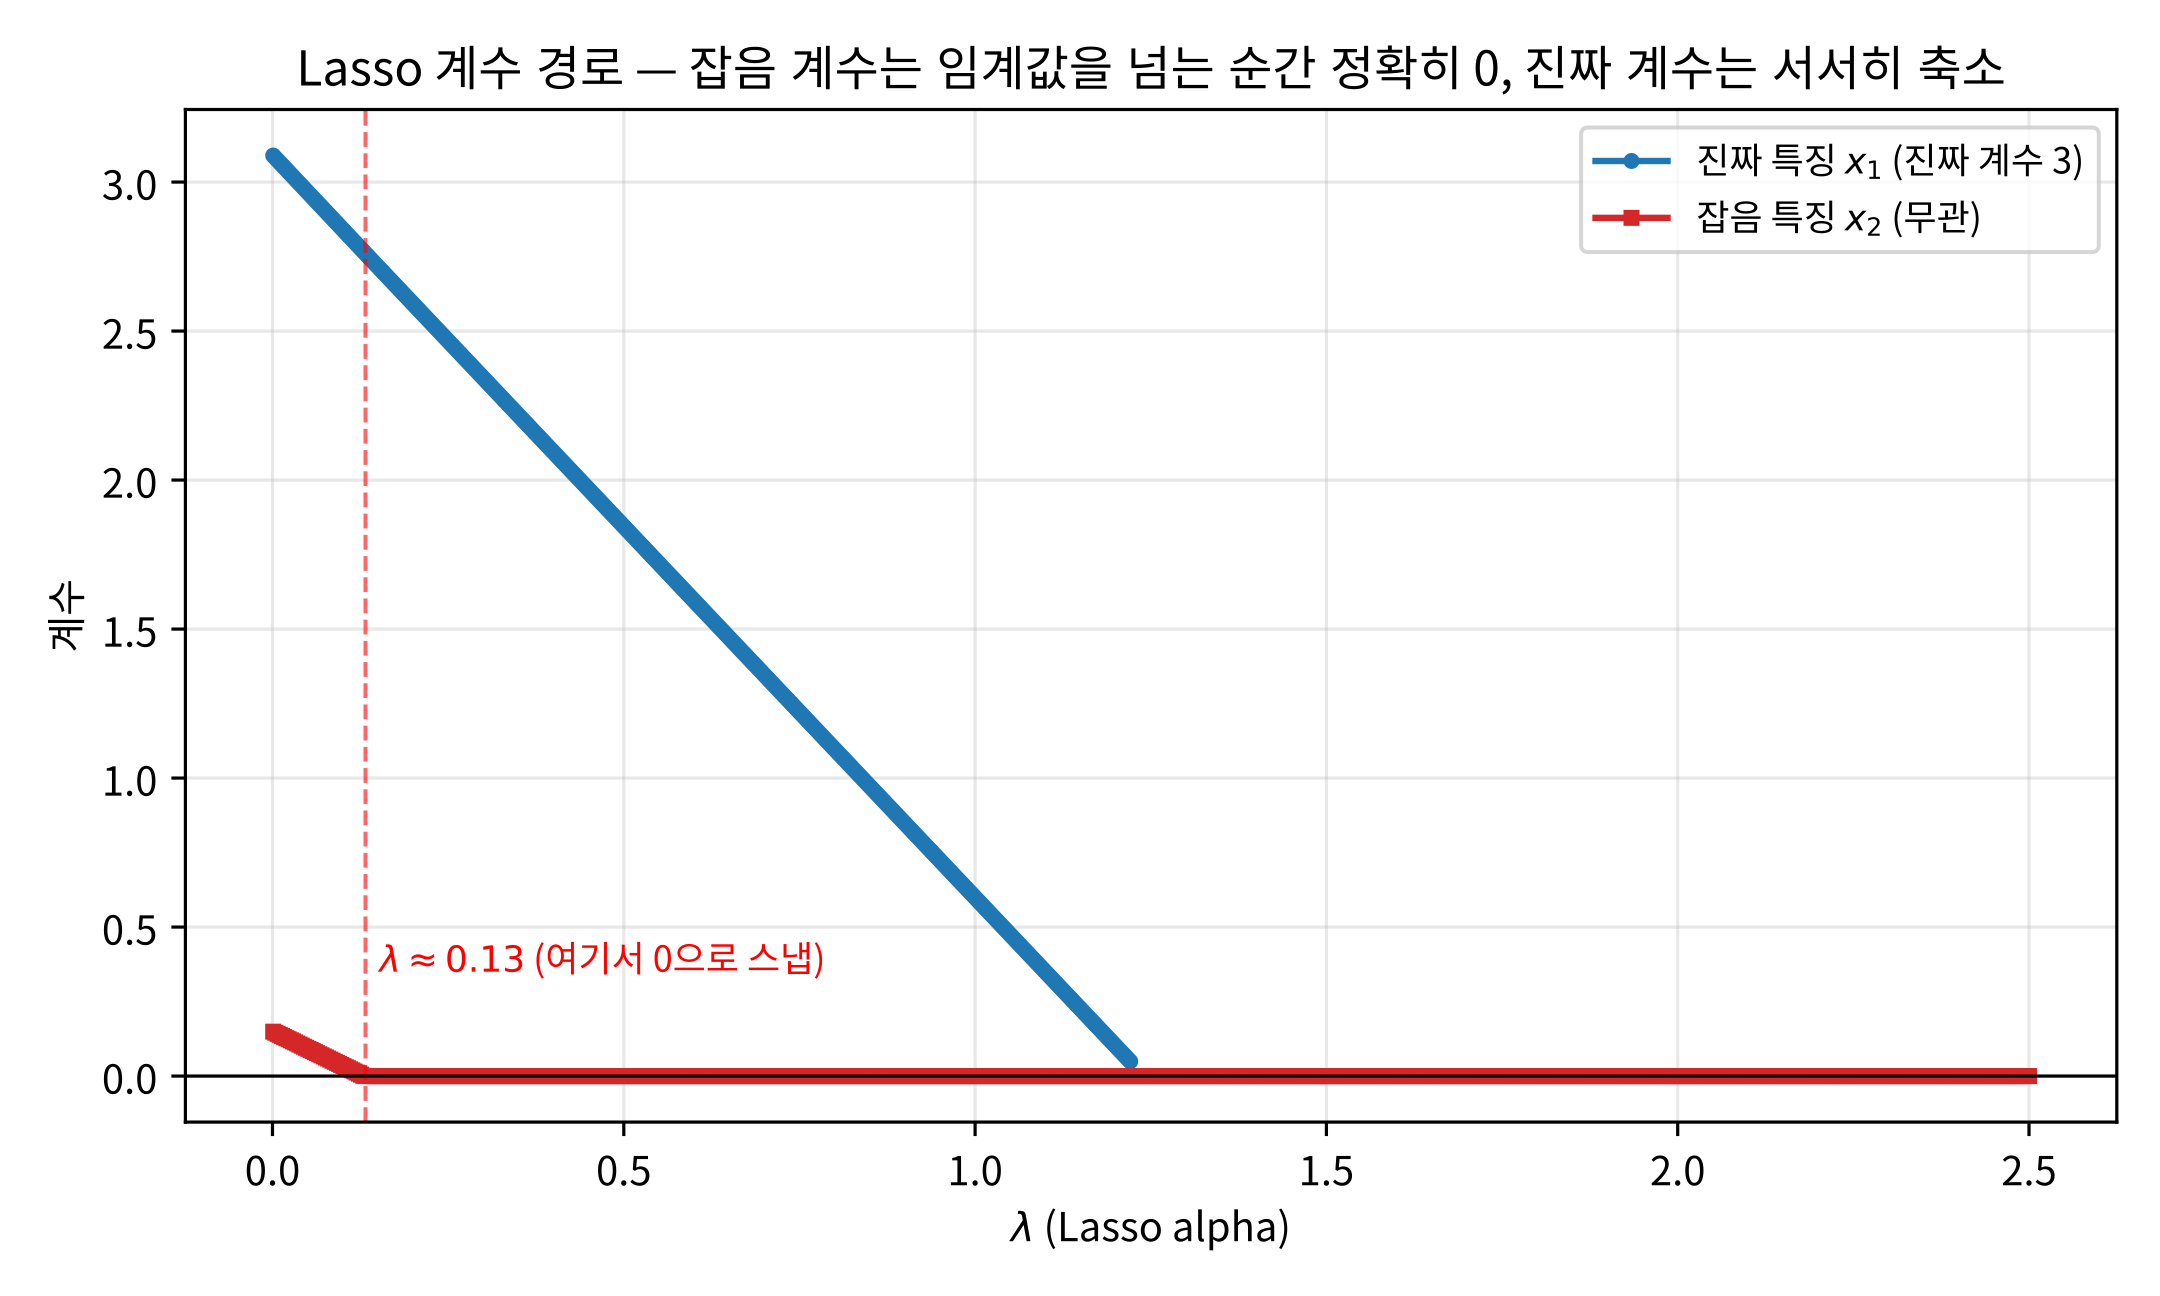
\includegraphics[width=0.5\linewidth]{ch06_1_lasso_path.png}
  \end{center}
  {\footnotesize \kb{LARS}(Least Angle Regression, Efron 등 2004): Lasso 해가
  $\lambda$에 대해 구간별로 선형이라는 성질 이용해 모든 $\lambda$의 계수를
  \emph{한 번에} 구하는 표준 알고리즘.}
\end{frame}

\begin{frame}{기하학적 직관: 원 vs 마름모}
  제약 $R(w)\le t$에서 원래 손실을 최소화하는 문제로 다시 쓰면:
  \begin{itemize}
    \item \kb{L2}: 제약 영역은 \textbf{원}(구) — 등고선이 표면 어디든 만남.
    \item \kb{L1}: 제약 영역은 \textbf{마름모}(각 축에 뾰족한 꼭짓점) —
      등고선이 \textbf{꼭짓점}(어떤 좌표가 0인 지점)에서 만날 확률이 훨씬 높음.
  \end{itemize}
  \vskip0.4em
  \textbf{2차원 숫자}: $X=[1,2,3,4]$, $y=[3,5,7,9]$(직선 $y=2x+1$, OLS 해
  $(1,2)$)에서 제약 $t=2$:
  \small
  \begin{tabular}{@{}lll@{}}
    \toprule
    & 최적점 & SSE \\
    \midrule
    L2(원) & $(0.67,\ 1.88)$ — 둘 다 0 아님 & $\approx1.60$ \\
    L1(마름모) & $(0,\ 2.0)$ — $w_0$ 축 \textbf{꼭짓점} & $\approx4.00$ \\
    \bottomrule
  \end{tabular}
  \par\vskip0.5em\normalsize
  \begin{block}{차원이 클수록 희소해진다}
    2차원에선 꼭짓점이 4개뿐이지만 특징 $p$개면 $p$차원 정다면체로 변해
    꼭짓점(=어떤 좌표가 0인 점)이 \textbf{방대}해짐. 특징이 많을수록
    ``등고선이 꼭짓점에서 만남'' 확률이 커지므로, Lasso의 희소(sparse)한
    해는 \textbf{차원이 클수록 더 흔해진다}.
  \end{block}
\end{frame}

\begin{frame}{L1 최적점은 꼭짓점에 닿는다}
  \begin{center}
    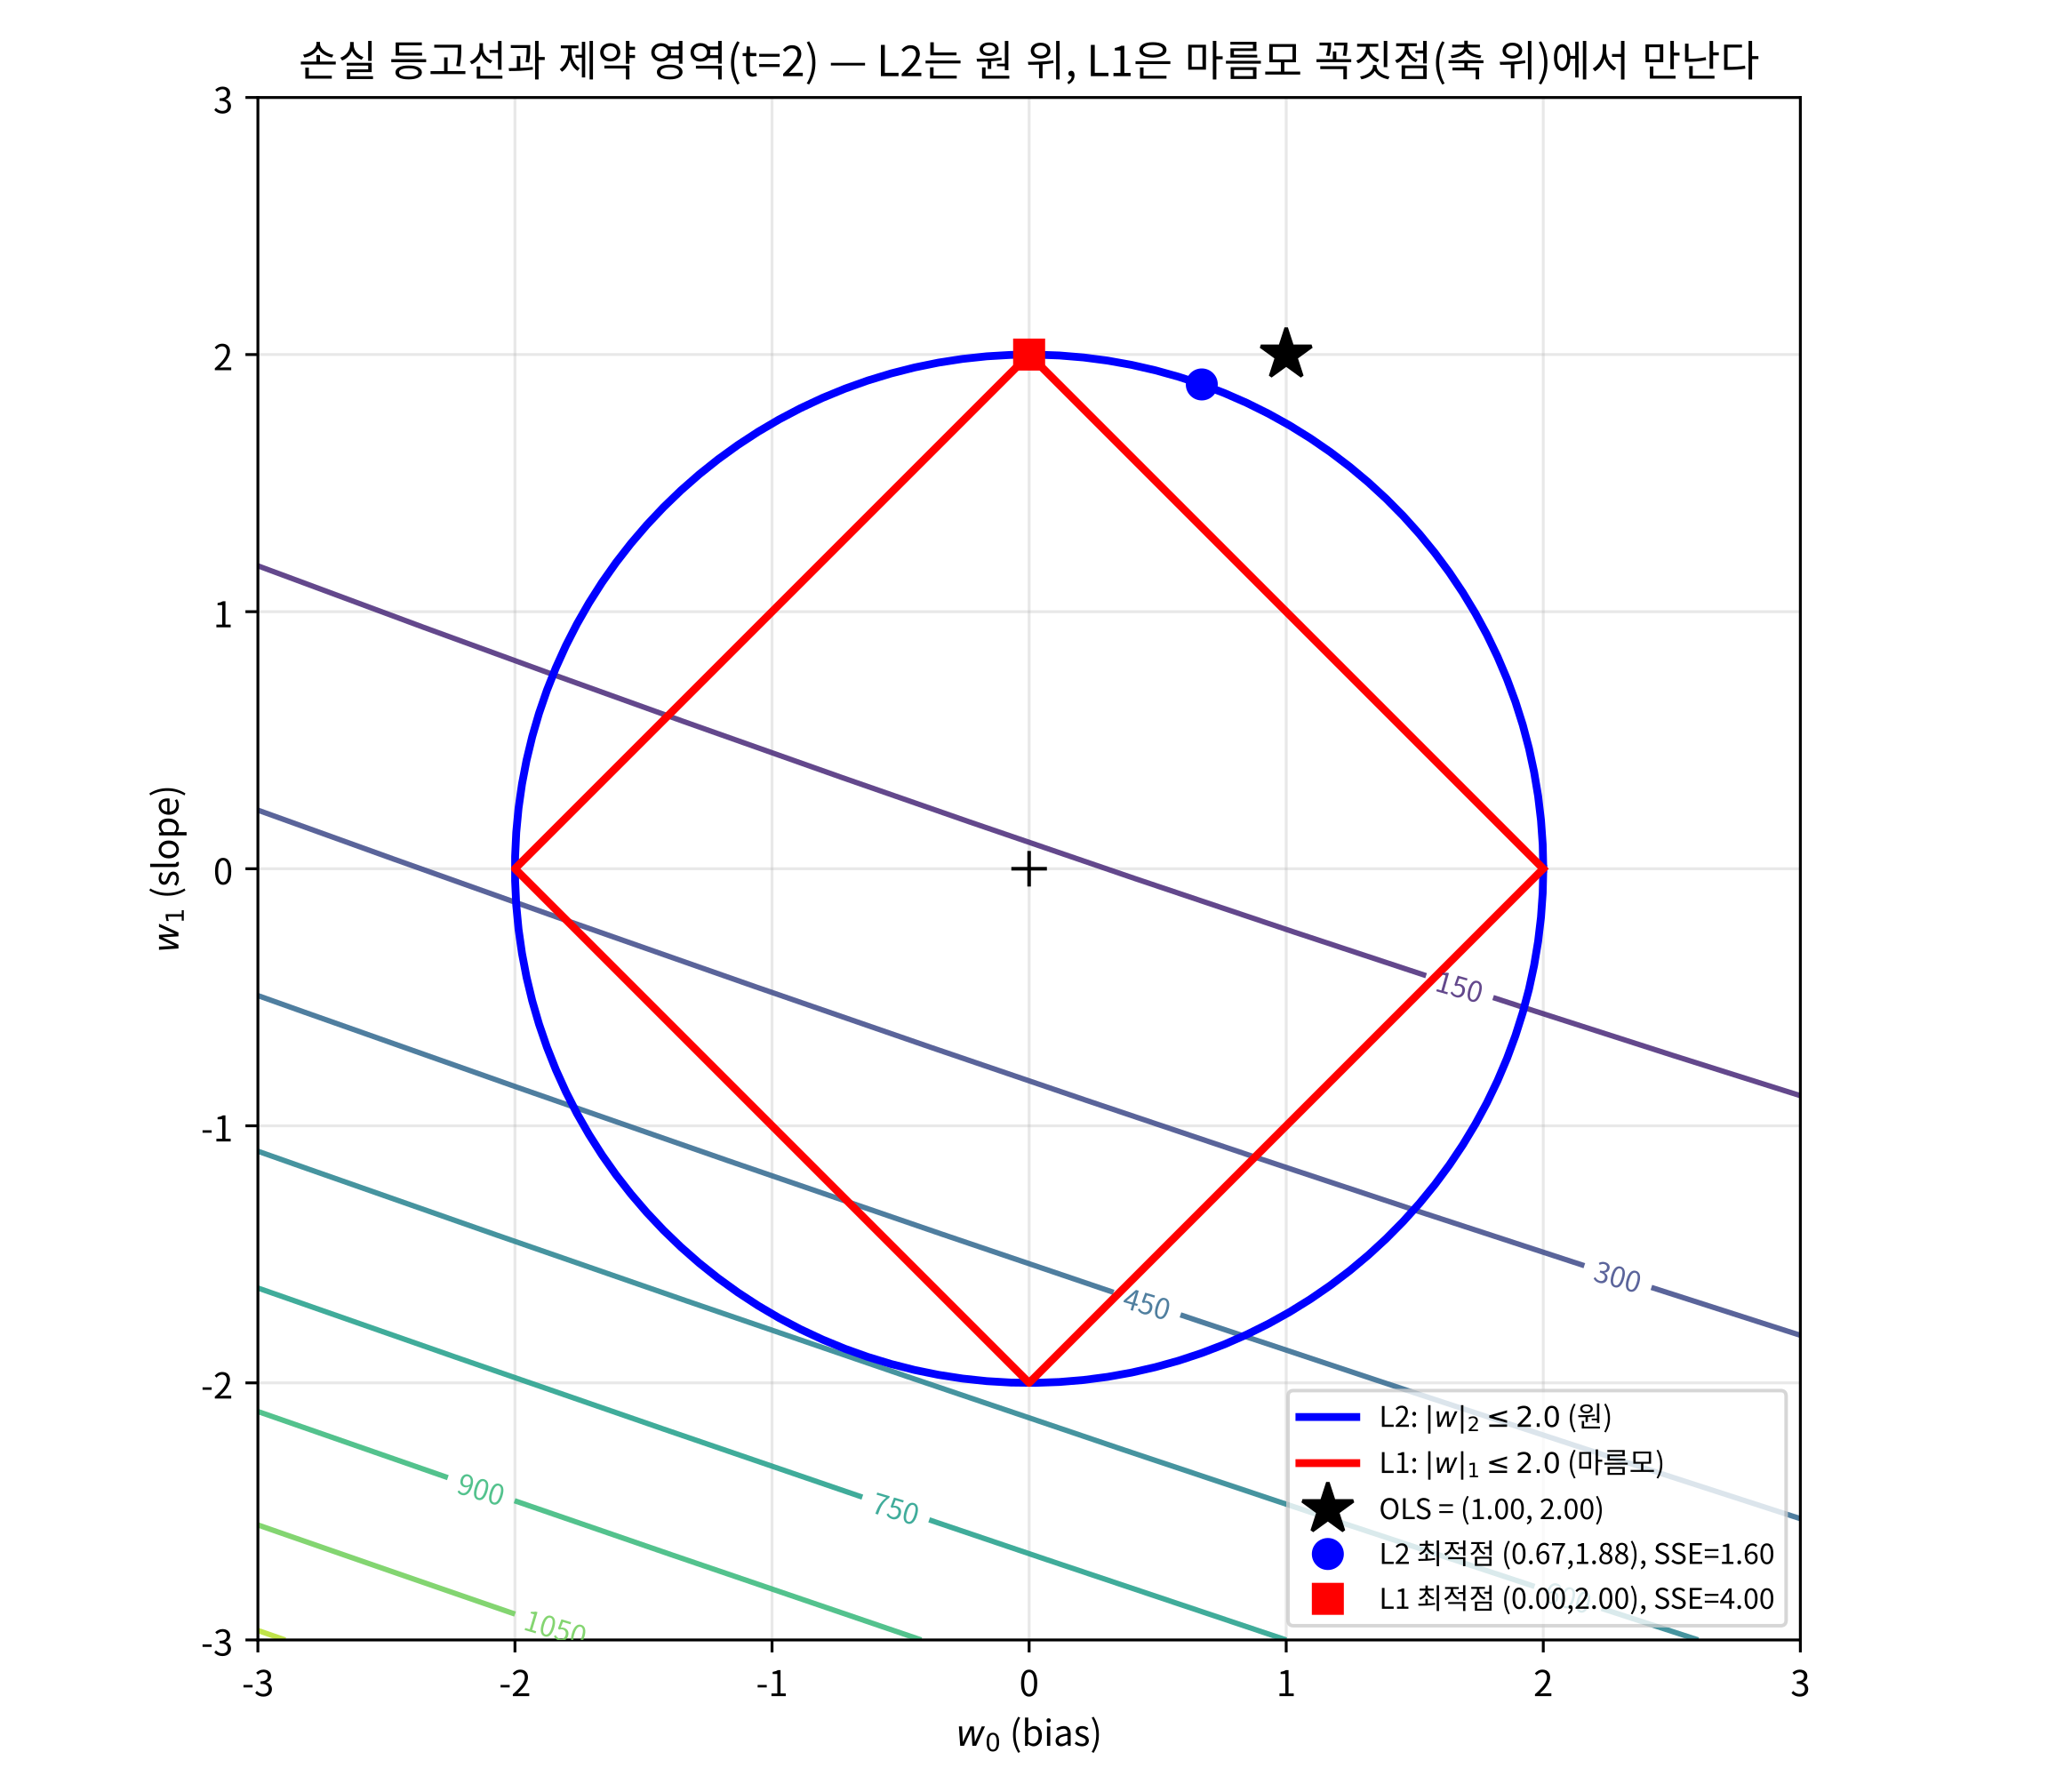
\includegraphics[width=0.58\linewidth]{ch06_1_l1_l2_geometry.png}
  \end{center}
  {\footnotesize 손실 등고선(타원)과 $t=2$인 원/마름모 — L2는 원 위의
  $(0.67,1.88)$에서, L1은 마름모 꼭짓점 $(0,2.0)$에서 만난다.}
  \vskip0.5em
  \begin{itemize}
    \item ``스냅''이 핵심: 계수가 0이면 ``매우 작은 숫자''가 아니라
      \textbf{모델 식에서 그 특징의 기여가 문자 그대로 0} — 그 특징을
      \emph{삭제해도} 예측이 한 치도 달라지지 않음.
    \item 특징이 수천 개인 실전에서 수백 계수가 \emph{정확히} 0이면 모델이
      자동으로 축소된 특징 목록으로 단순해진다.
    \item \textbf{주의}: 같은 $t$에서 L1의 SSE가 더 큰 것은 \emph{제약 크기}를
      고정하고 비교했기 때문. 실제로는 $\lambda$가 고정되고 각 방법이
      \emph{자기의} 최적점을 스스로 찾음.
  \end{itemize}
\end{frame}

\begin{frame}[fragile]{Ridge 경사하강 구현}
\begin{lstlisting}
def ridge_gradient_descent(X, y, lam, alpha, epochs):
    m, n = len(X), len(X[0])
    w = [0.0] * (n + 1)  # w[0] = bias
    for _ in range(epochs):
        grad = [0.0] * (n + 1)
        for i in range(m):
            pred = w[0] + sum(w[j+1] * X[i][j] for j in range(n))
            error = pred - y[i]
            grad[0] += error
            for j in range(n):
                grad[j+1] += error * X[i][j]
        for j in range(n + 1):
            # bias(w[0])는 관례적으로 정규화에서 제외
            reg = lam * w[j] if j > 0 else 0
            w[j] -= alpha * (grad[j] / m + reg)
    return w
\end{lstlisting}
  $\lambda$를 0에서 키우면 학습된 가중치가 0에 가까워짐 — 같은 데이터에
  $\lambda=0, 0.5, 5.0$을 넣으면 기울기 $w_1$이 $2.0 \to 1.4 \to 0.4$.
\end{frame}

\begin{frame}{손으로 한 번: Ridge 정규방정식}
  Ch.\,2.2의 정규방정식은 정규화 항이 있어도 닫힌 형태로 확장:
  \[
  w^{*} = (X^TX + \lambda D)^{-1}X^Ty \qquad (D\text{는 bias 제외 대각행렬})
  \]
  $X=[1,2,3]$, $y=[3,5,7]$(정규화 없는 해 $w^{*}=[1,2]$)에 $\lambda=2$:
  \[
  X^TX+\lambda D = \begin{bmatrix}3&6\\6&14\end{bmatrix} +
  \begin{bmatrix}0&0\\0&2\end{bmatrix} = \begin{bmatrix}3&6\\6&16\end{bmatrix}
  \]
  행렬식 $3\times16-6\times6=12$, $X^Ty=[15,34]$에 곱하면 $w^{*}=[3,\ 1]$.
  \vskip0.4em
  \begin{itemize}
    \item 기울기 $w_1$: $2\to1$ (``작게'' 만들려는 효과).
    \item bias $w_0$: $1\to3$으로 \textbf{커짐} — 기울기가 눌린 만큼 절편이
      데이터에 맞추며 보상.
    \item $\lambda=10$이면 $w^{*}\approx[4.33,\ 0.33]$으로 기울기가 더 0에
      가까워짐.
  \end{itemize}
\end{frame}

\begin{frame}{자주 하는 실수: bias(절편)까지 정규화}
  코드가 \texttt{reg = lam*w[j] if j > 0 else 0}로 bias를 굳이 건너뛰는
  이유. bias까지 정규화($D=I$)하면 같은 $\lambda=2$에서
  $w^{*}\_{\text{wrong}}=(X^TX+2I)^{-1}X^Ty\approx[0.818,\ 1.818]$ — bias가
  1에서 0.818로 \textbf{불필요하게} 끌려 내려감.
  \small
  \begin{tabular}{@{}lll@{}}
    \toprule
    $\lambda$ & 올바른 $D=\mathrm{diag}(0,1)$ & 틀린 $D=I$(bias도 정규화) \\
    \midrule
    2 & $[3.00,\ 1.00]$ & $[0.82,\ 1.82]$ \\
    10 & $[4.33,\ 0.33]$ & $[0.57,\ 1.28]$ \\
    \bottomrule
  \end{tabular}
  \par\vskip0.5em\normalsize
  \begin{block}{왜 안 좋은가}
    bias는 ``모델 복잡함''이 아니라 데이터 전체의 \textbf{평균적 높이}.
    기울기가 눌리면 bias가 \emph{보상하며 더 커져야} 한다(3.00$\to$4.33)는데,
    bias까지 정규화하면 $\lambda$가 커질수록 0 쪽으로 \emph{반대 방향}으로
    끌려가(0.82$\to$0.57) $y$의 평균이 원점에서 먼 데이터(주택 가격)에서
    체계적으로 \emph{아래}로 치우친다.
  \end{block}
  {\footnotesize scikit-learn \texttt{Ridge}, \texttt{Lasso} 등은 기본적으로
  bias/intercept를 정규화 대상에서 제외.}
\end{frame}

\begin{frame}{유명한 사례: Lasso는 유전체학에서 태어났다}
  1996년 티브시라니 논문에서 이 방법을 검증한 데이터가 바로
  \textbf{유전자 발현(genomics) 데이터}.
  \begin{itemize}
    \item 수백 개의 후보 유전자 중 실제 발현에 관여하는 소수를 ``수동으로''
      고르는 것은 불가능에 가까움.
    \item 특징 수(수백)가 샘플 수에 버금가는 문제에서, Lasso가 몇 개의
      유전자만을 \textbf{정확히 0이 아닌} 계수로 남김.
    \item 이 ``특징이 많고 진짜 신호는 소수'' 문제 구조는 30년 뒤에도
      그대로 — 전장 유전체 연관 분석(수백만 SNP에서 원인 변이), 희소 신호
      추정, 텍스트(수십만 단어 중 일부만 관련).
  \end{itemize}
  \vskip0.3em
  {\footnotesize Lasso 계열이 1차 후보로 쓰이는 이유: soft-thresholding이
  약한 계수를 0으로 스냅하는 성질 그 자체.}
\end{frame}

\begin{frame}[fragile]{실습: L1과 L2의 ``정확히 0'' 차이}
  \small
\begin{lstlisting}
from sklearn.linear_model import Ridge, Lasso
x1 = np.array([1,2,3,4,5,6], dtype=float)
x2 = np.array([5,3,8,1,9,2], dtype=float)   # y와 무관한 잡음
y  = 2 * x1 + 1
X  = np.column_stack([x1, x2])
for alpha in [0.1, 1.0, 5.0]:
    ridge = Ridge(alpha=alpha).fit(X, y)
    lasso = Lasso(alpha=alpha).fit(X, y)
    print(f"alpha={alpha}: ridge x2={ridge.coef_[1]:.4f}, "
          f"lasso x2={lasso.coef_[1]:.4f}")
\end{lstlisting}
\begin{columns}[T]
  \begin{column}{0.5\textwidth}
    \kb{Ridge}: $x_2$ 계수는 점점 작아지지만
    \textbf{정확히 0이 아님}
    (-0.0004 $\to$ -0.0040 $\to$ -0.0153)
  \end{column}
  \begin{column}{0.5\textwidth}
    \kb{Lasso}: 세 $\alpha$ 모두 $x_2$ 계수를 \textbf{정확히
    0.0000}으로 — 잡음 특징을 아예 ``제거''
  \end{column}
\end{columns}
  {\footnotesize 실전 데이터에서 Lasso가 이런 특징들의 계수를 0으로
  만들어주는 것이 곧 ``특징 선택을 자동으로 해낸다''의 실제 의미.}
\end{frame}

\begin{frame}[fragile]{한 뼘 더: 등가 특징 두 개면 어느 쪽을 남기는가}
  \small
  $x_1$과 \emph{완전히 같은 정보}를 담는 등가 특징 $x_{2c}=3x_1-4$(완전
  상관)를 추가 + 잡음 $x_3$:
\begin{lstlisting}
x2c = 3 * x1 - 4.0            # x1과 등가(완전 상관) 특징
x3  = np.array([2,9,1,7,3,6], dtype=float)
Xc  = np.column_stack([x1, x2c, x3])
print(Lasso(alpha=2.0).fit(Xc, y).coef_)
# [0. 0.5905 0.]   (순서: [x1, x2c, x3])
\end{lstlisting}
  놀라운 결과: Lasso는 \textbf{진짜 계수 2를 가진 $x_1$을 0으로 만들고},
  등가인 $x_{2c}$를 남김(계수 0.59, 환산 기울기 $\approx1.77$).
  \vskip0.3em
  ``어느 쪽을 남길지''는 \textbf{데이터가 결정하지 않는다} — 등가이면
  손실함수가 그 방향으로 평탄해져 해가 유일하지 않고, 솔버가 어느 꼭짓점에
  먼저 닿느냐에 따라 둘 중 하나가 \emph{임의로} 낙점.
  \vskip0.2em
  {\footnotesize 대조: Ridge는 상관 특징들의 가중치를 \emph{나눠 갖고}, Lasso는
  하나를 \emph{통째로 삭제} — 안정적 해 vs 희소 해, 둘 다 ``합법적''.}
\end{frame}

\begin{frame}{$\lambda$는 편향-분산 트레이드오프 위의 ``손잡이''}
  Ch.\,4.1의 분해(다시 인용). kNN의 유연도 손잡이가 $k$였다면 선형모델의
  손잡이는 $\lambda$:
  \[
  \mathbb{E}\left[(y - \hat f(x))^2\right] =
  \underbrace{\left(\text{Bias}[\hat f(x)]\right)^2}_{\text{구조적으로 못 맞추는 정도}}
  + \underbrace{\text{Var}[\hat f(x)]}_{\text{훈련이 바뀔 때 예측이 흔들림}}
  + \underbrace{\sigma^2}_{\text{데이터의 잡음}}
  \]
  4.1의 수치 실험($f^{*}(x)=\sin(2\pi x)$, 잡음 $\sigma=0.5$, 100점,
  300회 재추출)과 \textbf{완전히 같은 방식}으로 재측정. 이번엔 모델이
  \textbf{15차 다항식}(충분히 유연, $\lambda=0$이면 100점을 거의 통과),
  ``유연도 줄이는 조작''이 $\lambda$를 올리는 것.
\end{frame}

\begin{frame}{숫자로 확인: $\lambda$ 축을 훑는다}
  \small
  \begin{tabular}{@{}rrrr@{}}
    \toprule
    $\lambda$ & $\text{Bias}^2$ & $\text{Var}$ & test RMSE \\
    \midrule
    0     & 5.64  & 110.90 & 10.81 \\
    0.001 & 0.24  & 0.030  & 0.66 \\
    0.01  & 0.26  & 0.015  & 0.68 \\
    0.1   & 0.40  & 0.008  & 0.80 \\
    1.0   & 0.44  & 0.004  & 0.85 \\
    10    & 0.48  & 0.004  & 0.88 \\
    100   & 0.49  & 0.004  & 0.89 \\
    \bottomrule
  \end{tabular}
  \par\vskip0.5em\normalsize
  \begin{itemize}
    \item \kb{$\lambda=0$}: ``주사위''처럼 출렁. $\text{Var}=110.9$로 극도로
      크고 RMSE 10.81은 \textbf{잡음 플로어(0.88)의 12배}. 과적합이
      $\lambda$ 축의 \emph{왼쪽 끝}.
    \item \kb{$\lambda=0.001$}: Var 110.9$\to$0.03으로 4자릿수 급감, Bias²
      0.24로 아직 작음. RMSE 0.66 = \textbf{곡선의 바닥}. ``분산 제거''에
      \textbf{극도로 효율적}.
    \item \kb{$\lambda=100$}: 가중치 완전히 눌려 ``훈련 평균값만 내뱉는''
      수준. Bias² 0.49, RMSE 0.89로 잡음 플로어에 붙음 —
      ``$\lambda\to\infty$이면 평균값만 예측하는 모델''의 숫자 확인.
  \end{itemize}
\end{frame}

\begin{frame}{U자형 곡선과 잡음 플로어}
  \begin{center}
    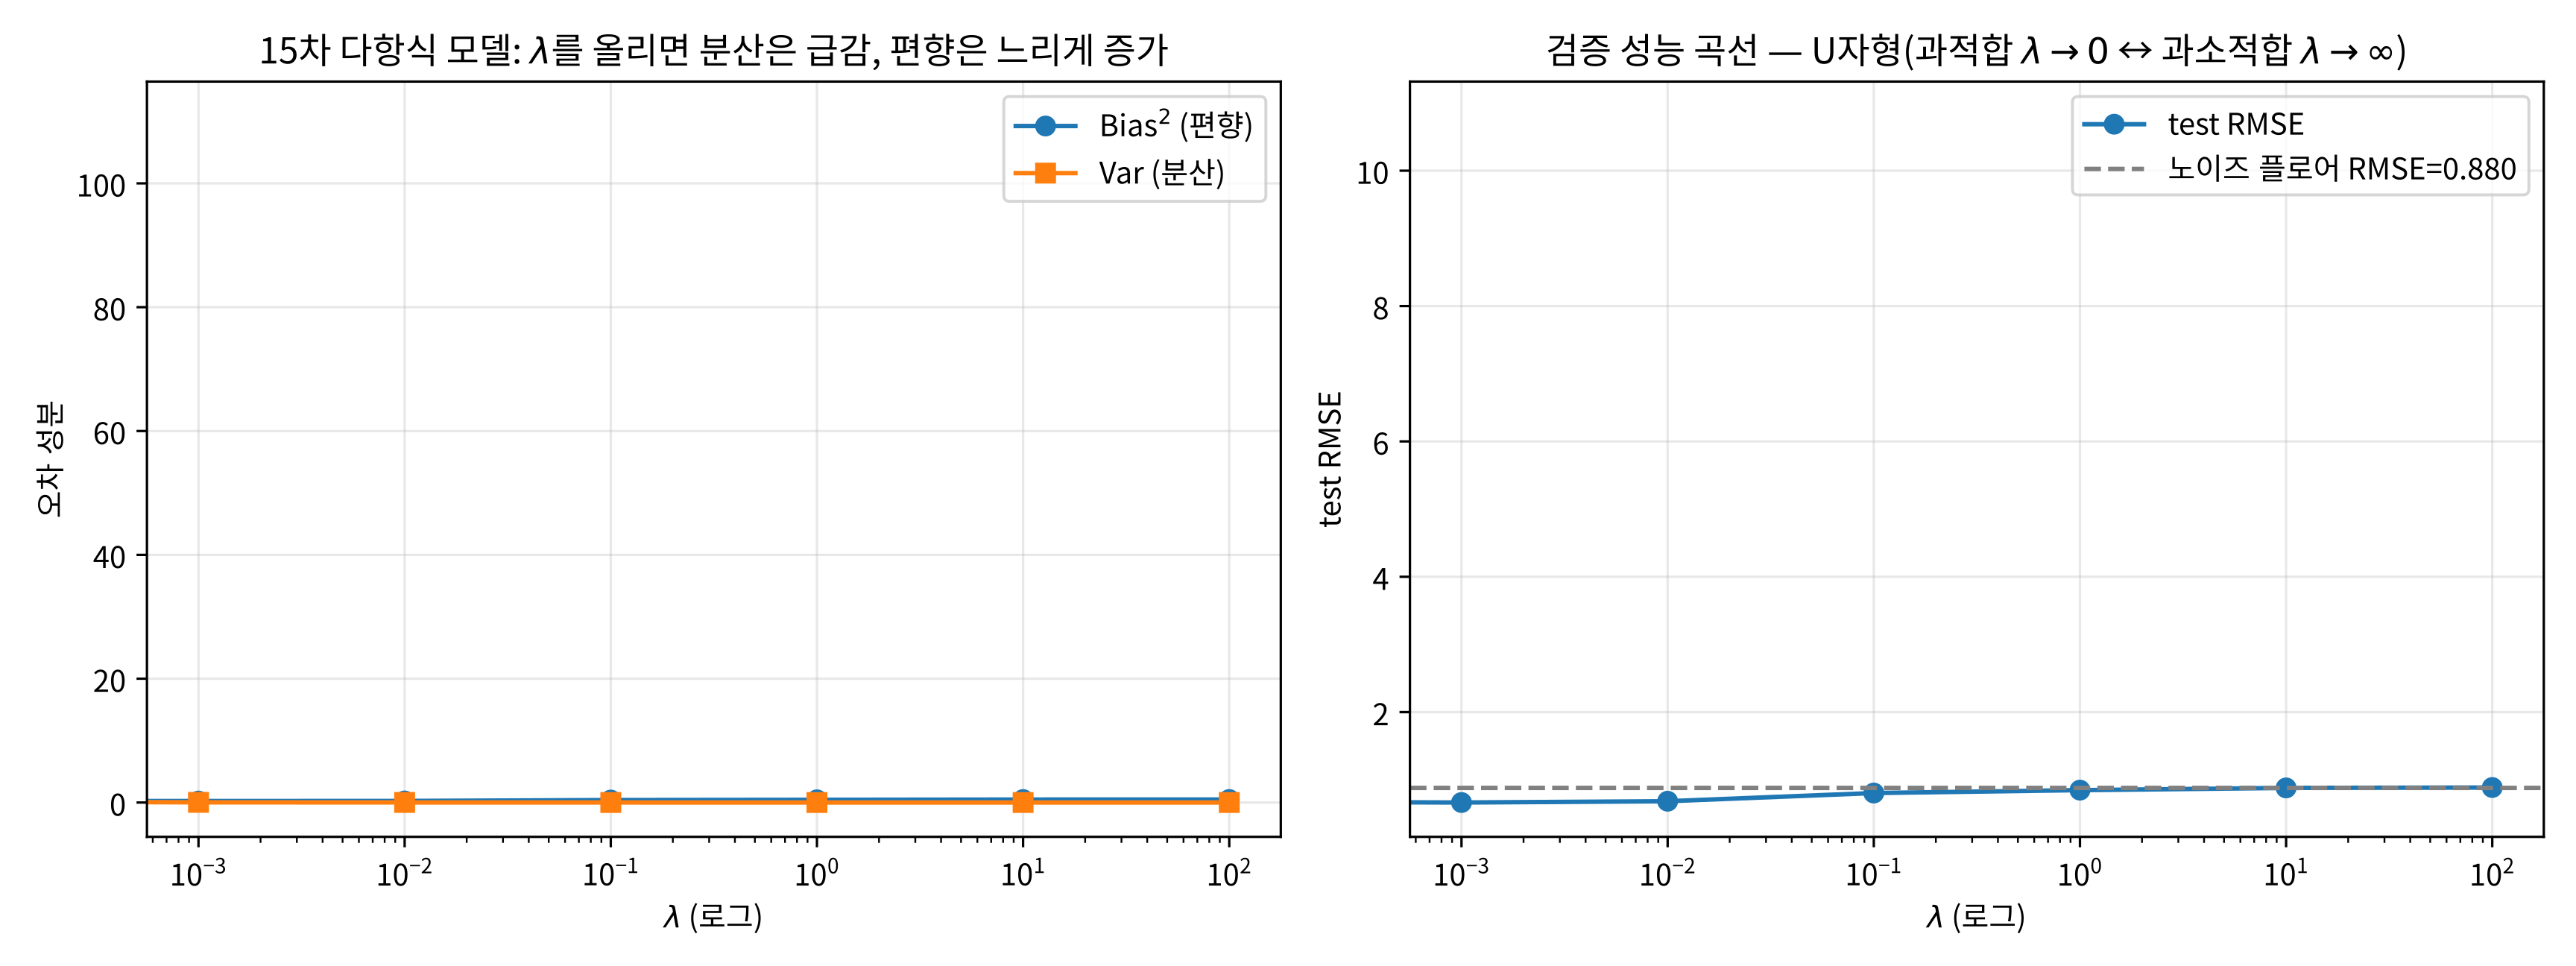
\includegraphics[width=0.62\linewidth]{ch06_1_lambda_biasvar.png}
  \end{center}
  {\footnotesize 좌측: $\lambda$(로그 축)에 따른 Bias²와 Var — Var는
  $\lambda$를 올리자 급감, Bias²는 느리게 상승. 우측: test RMSE 곡선(U자형)과
  잡음 플로어(0.88, 회색 점선).}
  \vskip0.4em
  \begin{block}{U자형 곡선}
    왼쪽 날개 = 과적합(Var 지배), 오른쪽 날개 = 과소적합(Bias² 지배),
    바닥 = 최적 $\lambda$의 \emph{대략적} 위치.
  \end{block}
  \kq{이 U자의 바닥을 ``정직하게'' 찾는 방법 = 6.2(교차검증)의 존재 이유.
  검증 데이터가 없으면 ``아마 이 부근''까지만 알 수 있다.}
\end{frame}

\begin{frame}{자주 묻는 질문 (1)}
  \textbf{Q. 항상 Lasso(L1)를 쓰는 게 낫나요?}
  \begin{itemize}
    \item 아님. 특징이 강하게 상관되면(집 크기 대 방 개수) Lasso는 하나만
      임의로 남기고 나머지를 0으로 — \textbf{불안정}(데이터 살짝 바꿔도
      남는 특징이 달라질 수 있음).
    \item Ridge는 상관 특징들의 가중치를 비슷하게 나눠 갖는 경향 →
      \textbf{안정적}.
    \item 실전: 둘을 섞은 \kb{엘라스틱넷}(Zou·Hastie 2005),
      $R(w) = \alpha\|w\|_1 + (1-\alpha)\|w\|_2^2$.
  \end{itemize}
  \vskip0.4em
  \textbf{Q. Lasso가 0으로 만든 특징이 사실 중요했지만 효과 작아
  떨어진 경우, 어떻게 구별?}
  \begin{itemize}
    \item 구분할 \emph{수 없는} 것이 정답에 가까움 — $w_j=0$은 ``무관하다''는
      증명이 아니라 \emph{그 $\lambda$에서} 최적화가 내린 \textbf{선택의 결과}.
    \item 진짜 계수 3이면 $\lambda=0.13$ 넘겨도 살아남지만 0.2였으면 같은
      $\lambda$에서 0 — 신뢰도는 ``진짜 계수 $>$ 임계 $\lambda$'' 전제에
      달려 있고, 그 전제는 데이터 이전에 보장되지 않음.
    \item 줄이는 법: 특징 \textbf{스케일링} + $\lambda$를 6.2의 CV로
      ``너무 크게'' 잡지 않게.
  \end{itemize}
\end{frame}

\begin{frame}{자주 묻는 질문 (2)}
  \textbf{Q. $\lambda$가 너무 크면?}
  \begin{itemize}
    \item $\lambda\to\infty$이면 정규화 항이 원래 손실을 압도 →
      모든 가중치(bias 제외)가 0에 수렴, ``항상 평균값만 예측하는'' 가장
      단순한 모델로 수렴(분산 $\to$0, 편향 극도로 큼 = 과소적합 극단).
  \end{itemize}
  \vskip0.4em
  \textbf{Q. $|w|$가 미분불가능하면 Lasso는 최적화할 수 없는 거 아닌가요?}
  \begin{itemize}
    \item 아님 — 0에서의 서브그래디언트($[-1,1]$)로 최적조건을 정의하면
      해가 존재하고 \textbf{좌표하강}이 효율적으로 찾음.
    \item L2는 모든 점에서 미분가능 → 구배하강·닫힌형 모두 가능. Lasso는
      0에서 뾰족 → 전용 알고리즘(좌표하강·내적점). 실전에서 \texttt{Lasso}를
      그냥 \texttt{.fit()}하는 것은 이 전용 알고리즘을 쓰는 것.
  \end{itemize}
  \vskip0.4em
  \textbf{Q. 정규화 계수 $\lambda/2$ vs $\lambda$, sklearn \texttt{alpha}?}
  \begin{itemize}
    \item 기호가 서로 다름($\frac{\lambda}{2m}\|w\|^2$,
      $\frac{\lambda}{2}\|w\|^2$, $\lambda\sum w_j^2$). sklearn
      \texttt{Ridge(alpha=a)}는 $\frac{a}{2}\sum w_j^2$.
    \item \textbf{상대적 강도만} 의미 있고 절대값은 무의미 → 다른
      라이브러리의 $\lambda$를 \emph{숫자로} 비교하지 말 것. ``적절한 강도''
     는 6.2의 CV로 \textbf{데이터가} 정한다.
  \end{itemize}
\end{frame}

\begin{frame}{확인 문제 6.1}
  \small
  \begin{enumerate}
    \item \textbf{참}인 것을 모두 고르라: (a) Ridge에서 $\lambda\to0$이면 해는
      OLS로 수렴. (b) Lasso에서 $\lambda\to\infty$이면 bias 제외 모든 계수
      정확히 0. (c) Lasso는 항상 $y$와 상관 큰 특징만 남김.
      (d) L1/L2의 ``적당한'' $\lambda$는 train loss가 가장 작은 곳에서 고른다.
      \newline\newline
      {\footnotesize 힌트: (c)는 등가 특징 예, (d)는 6.2 서두 ``train loss만
      보면 항상 $\lambda=0$''}
    \item \textbf{soft-thresholding 손계산.} $f(w)=\frac12(2-w)^2+\lambda|w|$에서
      $\lambda=0.5$와 3일 때 최적 해를 $\mathcal{T}_\lambda(z)$($z=2$)로 구하고,
      ``왜 0이 되고/안 되는지'' $|z|\le\lambda$ 조건으로 설명.
    \item \textbf{서브그래디언트.} $|w|$의 $w_0>0, w_0<0, w_0=0$에서
      서브그래디언트($1, -1, [-1,1]$)를 구하고, $f(w)=\frac12(z-w)^2+\lambda|w|$에
      대해 $w^{*}=0 \iff |z|\le\lambda$를 증명한 뒤 $|z|>\lambda$일 때
      $w^{*}=\text{sign}(z)(|z|-\lambda)$ 확인(soft-thresholding의 \emph{증명}).
    \item \textbf{개념.} 등가 특징 예에서 Lasso가 $x_1$ 대신 $x_{2c}$를
      남긴 이유를 L1 페널티 관점에서 설명(힌트: 같은 예측 만드는
      $(w_1,w_{2c})$ 중 어느 쪽이 $|w_1|+|w_{2c}|$가 작나).
  \end{enumerate}
\end{frame}

\begin{frame}{6.1 정리}
  \begin{itemize}
    \item 정규화는 손실함수에 ``가중치 크기'' 페널티 한 항을 더해 유효 유연성을
      낮춤 — 4.1의 언어로 $\lambda$를 올리면 \textbf{분산을 편향과 바꾸는} 것.
      살짝만 올려도 Var가 4자릿수 급감할 만큼 ``분산 제거''에 효율적.
    \item L2는 모든 가중치를 \textbf{매끄럽게} 축소, L1은
      soft-thresholding($|z_j|\le\lambda$이면 0)으로 약한 특징을
      \textbf{정확히 0}에 스냅시켜 특징 선택을 \emph{무상}으로 —
      기하학적으로 ``원 위'' vs ``마름모 꼭짓점 위''.
    \item bias는 관례적으로 정규화 대상에서 \textbf{제외}.
  \end{itemize}
  \vskip0.4em
  \kq{``$\lambda$ 자체는 얼마가 적정한가'' — U자형 곡선의 바닥을 정직하게
  고르는 절차는 6.2(교차검증)·6.3(train/val/test)에서.}
\end{frame}

% =====================================================================
\section{6.2 교차검증: $\lambda$를 데이터로 정한다}

\begin{frame}{왜 검증 데이터가 필요한가}
  $\lambda$는 사람이 직접 정해야 하는 \kb{하이퍼파라미터} —
  학습으로 정해지는 $w$와 달리, 학습 \emph{시작 전에} 값을 정해줘야
  하는 파라미터.
  \begin{itemize}
    \item 학습 데이터 손실만 보고 고르면 \textbf{항상 $\lambda=0$}
      (정규화 없음)이 제일 낮은 손실을 냄 → 의미 없음.
    \item \textbf{검증 데이터}(validation set)로 성능을 재야 한다.
  \end{itemize}
  \vskip0.5em
  \begin{block}{데이터가 넉넉하지 않을 때: k-겹 교차검증}
    \kb{k-겹 교차검증}(k-fold cross-validation): 데이터를 $k$개로 쪼갠
    뒤, 매번 한 조각을 검증용으로 남기고 나머지로 학습하는 것을 $k$번
    반복해 성능을 평균냄 — 전체를 \emph{한 번씩은} 검증에도 학습에도
    써보는 셈.
  \end{block}
\end{frame}

\begin{frame}[fragile]{k-fold 분할 코드}
\begin{lstlisting}
def k_fold_split(data, k, fold_idx):
    n = len(data)
    fold_size = n // k
    start = fold_idx * fold_size
    end = start + fold_size if fold_idx < k - 1 else n
    val   = data[start:end]
    train = data[:start] + data[end:]
    return train, val
\end{lstlisting}
  \begin{itemize}
    \item \texttt{fold\_idx}번째 블록을 검증용(val), 나머지를 학습용(train)
      반환. 마지막 fold는 남은 것을 전부 포함.
    \item \kq{주의: 주어진 \emph{순서 그대로} 앞에서부터 자름 — 정렬된
      데이터는 §자주 하는 실수 참조.}
  \end{itemize}
  {\footnotesize 실전 \texttt{KFold(shuffle=True)} 또는 클래스 비율을
  유지하는 \texttt{StratifiedKFold} 권장.}
\end{frame}

\begin{frame}{손으로 한 번: ``아무것도 못 배우는'' 모델 5-fold CV}
  검증 성능이 어떤 숫자가 ``합리적인지'' 감각을 위해, 가장 단순한 모델 —
  \textbf{학습 데이터의 평균만 되뇐다}(평균모델) — 로 5-fold CV를
  손계산. $y=1,2,\dots,10$을 순서대로 2개씩 5등분:
  \small
  \begin{tabular}{@{}llrl@{}}
    \toprule
    fold & val & train 평균 & fold별 MSE \\
    \midrule
    0 & 1, 2   & 6.5 & 25.25 \\
    1 & 3, 4   & 6.0 & 6.50 \\
    2 & 5, 6   & 5.5 & 0.25 \\
    3 & 7, 8   & 5.0 & 6.50 \\
    4 & 9, 10  & 4.5 & 25.25 \\
    \midrule
    & \multicolumn{2}{r}{\textbf{평균}} & \textbf{12.75} \\
    \bottomrule
  \end{tabular}
  \par\vskip0.5em\normalsize
  fold 0 풀어쓰기: train $=\{3,\dots,10\}$의 평균 $=(3+\cdots+10)/8=6.5$,
  $\text{MSE}=[(1-6.5)^2+(2-6.5)^2]/2=[30.25+20.25]/2=25.25$.
  \vskip0.3em
  {\footnotesize ``정직한'' 기준선: 진짜 평균 5.5로 예측했을 때의 MSE $=\frac{82.5}{10}=8.25$.}
\end{frame}

\begin{frame}{CV 추정값은 ``진짜 성능''이 아니다}
  \begin{block}{CV 추정값(12.75)이 정직한 값(8.25)보다 53\%나 높다}
    각 fold의 ``train 평균''(6.5, 6.0, 5.5, 5.0, 4.5)이 진짜 평균 5.5
    주위를 흔들리기 때문. train 평균이 1.0만큼 어긋난 fold 0에서 그
    어긋남이 val 오차에 \emph{그대로} 더쳐진다.
    \vskip0.3em
    \textbf{CV 추정값은 ``진짜 성능''이 아니라 ``검증 절차의 시뮬레이션''} —
    절차 안의 작은 흔들림도 포함되므로 특정 모델 하나엔 오히려
    \emph{높게}(비관적으로) 나올 수도.
  \end{block}
  \vskip0.4em
  \begin{itemize}
    \item ``CV 수치가 항상 낙관적''이라는 직관을 \textbf{바로잡}자 —
      \kq{CV의 낙관적 편향은 ``한 모델을 평가''할 때 생기는 게 아니라,
      ``여러 후보 중 \emph{제일 좋은} 모델을 고르는'' 다음 단계에서
      생긴다}(§최적화 편향).
    \item 모델 \emph{하나}를 단순히 평가하는 단계(여기처럼 유연하지
      않으면) — CV가 진짜 오차보다 \emph{낮게} 나올 리가 없고, 실제로
      \emph{높게} 나올 수도.
  \end{itemize}
\end{frame}

\begin{frame}[fragile]{k-fold CV로 최적 $\lambda$ 찾기}
  \small
\begin{lstlisting}
def cross_validate_lambda(X, y, lambdas, k=5, alpha=0.01, epochs=500):
    data = list(zip(X, y))
    results = {}
    for lam in lambdas:
        val_errors = []
        for fold in range(k):
            train, val = k_fold_split(data, k, fold)
            Xtr, ytr = [d[0] for d in train], [d[1] for d in train]
            Xva, yva = [d[0] for d in val],   [d[1] for d in val]
            w = ridge_gradient_descent(Xtr, ytr, lam, alpha, epochs)
            val_errors.append(mse(Xva, yva, w))
        results[lam] = sum(val_errors) / len(val_errors)
    return results
\end{lstlisting}
  ``학습 손실이 아니라 \textbf{검증 손실}로 $\lambda$를 고른다''는 원칙을
  코드로 확인.
\end{frame}

\begin{frame}{U자형이 실제로 그려진다}
  특징 15개 중 $y$와 관련 있는 건 2개뿐, 나머지는 순수 잡음. 실행 예:
  \small
  \begin{tabular}{@{}rl@{}}
    \toprule
    $\lambda$ & 평균 검증 MSE \\
    \midrule
    0.0  & 12.520 \\
    0.5  & 10.872  \textbf{← 최적} \\
    2.0  & 11.780 \\
    10.0 & 13.740 \\
    \bottomrule
  \end{tabular}
  \par\vskip0.5em\normalsize
  \begin{itemize}
    \item 정규화 전혀 없음($\lambda=0$)도, 너무 강함($\lambda=10$)도
      검증 MSE가 오히려 나빠지고, 그 사이 어딘가에 최적점.
    \item 이 U자 모양 = 6.1의 편향-분산 트레이드오프가 실제 숫자로
      나타난 것.
  \end{itemize}
  \vskip0.3em
  {\footnotesize 같은 종류의 데이터(15개 특징 중 2개 진짜, $n=100$, 잡음
  $\sigma=3$)에 로그 스케일 41개 후보를 밀게 돌려 그리면 모양이 선명.
  Ridge는 정규방정식으로 닫혀 있어 완전한 해로만 봄.}
\end{frame}

\begin{frame}{U자형 곡선: 좌측=과적합, 우측=과소적합}
  \begin{center}
    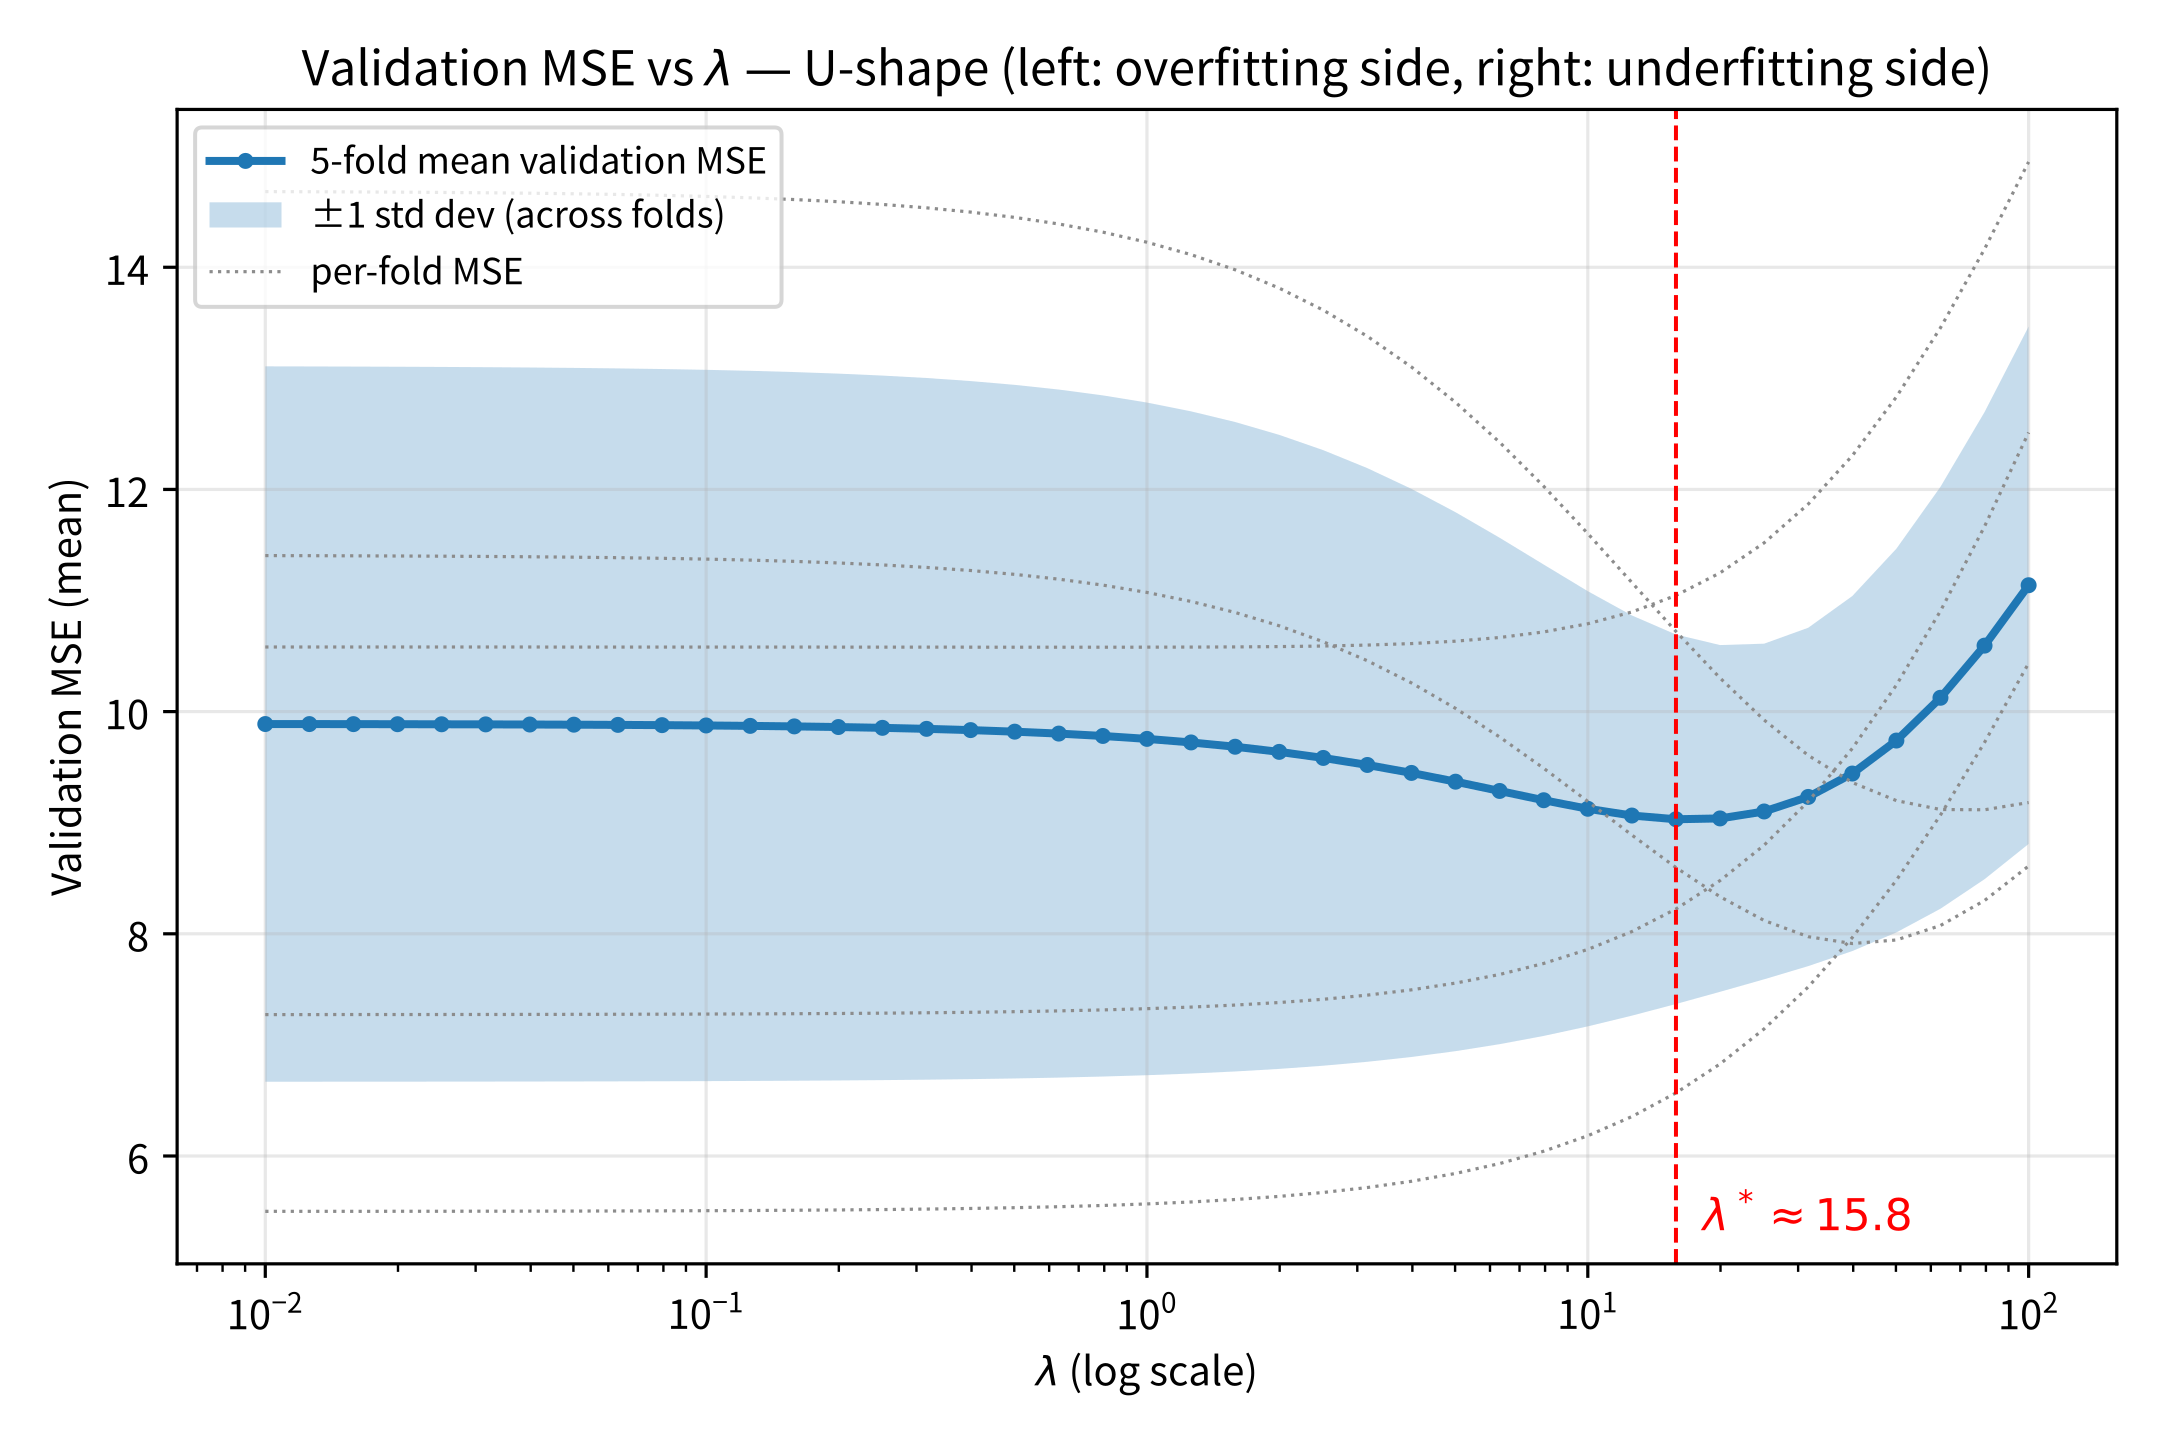
\includegraphics[width=0.62\linewidth]{ch06_2_lambda_ucurve.png}
  \end{center}
  {\footnotesize $\lambda$(로그 스케일)에 따른 5-fold 평균 검증 MSE — U자형.
  최소점 $\lambda^{*}\approx15.8$(MSE$\approx9.03$). 회색 점선 = fold별 MSE,
  막대 = $\pm1$ 표준편차 밴드.}
  \vskip0.4em
  \begin{itemize}
    \item \kb{U의 왼쪽}($\lambda$ 작음, 과적합): 13개 잡음 특징 가중치가
      표본잡음에 맞춰 \textbf{분산 지배}. $\lambda\to0$일수록 이 쪽 —
      정규화 없는 모델(12.520)은 최소점보다 나쁨.
    \item \kb{U의 오른쪽}($\lambda$ 큼, 과소적합): 2개 \emph{진짜} 관련
      특징 가중치까지 0으로 쪼그라들며 \textbf{편향} 커짐.
    \item \kb{최소점}: 둘의 합이 가장 작은 위치.
  \end{itemize}
  \vskip0.2em
  {\footnotesize 놓치기 쉬운 것: 평균 곡선이 U자형인 데다 \textbf{최소점
  근처로 갈수록 fold 간 흩어짐(밴드)도 좁아진다} — ``제일 낮은 한 점''을
  어디까지 믿을 수 있느냐의 문제.}
\end{frame}

\begin{frame}{1SE 규칙: 최소점은 뾰족한 꼭짓점이 아니다}
  \begin{itemize}
    \item CV 곡선의 ``최소점''은 \emph{추정치} — 데이터가 조금만 바뀌어도
      위치가 동네를 바꿈.
    \item 같은 생성 과정을 시드 10개로 반복하면 각 시드가 고른 $\lambda^{*}$가
      \textbf{5.0$\sim$20.0까지}(약 4배) 흩어짐 → \emph{평탄한 대지
      (plateau)}.
  \end{itemize}
  \vskip0.4em
  \begin{block}{\kb{1SE 규칙}(1-standard-error rule, Tibshirani 1996)}
    CV MSE가 (\textbf{최소점 + fold 표준편차 1개}) 이내인 후보 중
    \textbf{가장 큰 $\lambda$} — 즉 \textbf{가장 단순한 모델} — 을 고른다.
    \vskip0.3em
    논리: ``CV 평균의 불확실성은 $\pm1$ 표준편차 급이고, 그 범위 안에서는
    더 단순한 쪽을 고르는 것이 합리적 tie-breaker''.
  \end{block}
\end{frame}

\begin{frame}{1SE 규칙 적용: 5배 큰 $\lambda$}
  위 곡선에서 계산:
  \begin{itemize}
    \item 최소점 $\lambda\approx15.8$(MSE 9.03), fold 표준편차 1개(1.66)를
      더한 허용 상한 = \textbf{10.69}.
    \item 이 범위 안에 드는 후보 중 가장 큰 $\lambda$ =
      \textbf{$\lambda\approx79.4$}(MSE 10.59) — 최소점보다 \textbf{5배}
      더 큰 $\lambda$.
  \end{itemize}
  \vskip0.5em
  \begin{block}{실전 의미}
    더 작고 단순한 모델이 ``통계적으로 구별되지 않는'' 수준으로 좋다.
    6.1의 Lasso로 치면, 정확도를 사실상 그대로 유지하면서 \emph{더 많은}
    특징을 0으로 만들어 \textbf{더 희소하고 해석하기 쉬운} 모델을 얻음.
  \end{block}
\end{frame}

\begin{frame}{손으로 한 번: 4-fold 분할 직접 나눠보기}
  \small
  샘플 12개(인덱스 0$\sim$11)를 $k=4$로 나누면 \texttt{fold\_size}=12//4=3.
  각 \texttt{fold\_idx}에 대해 \texttt{start}=\texttt{fold\_idx$\times$3},
  \texttt{end}=\texttt{start+3}(마지막 fold만 $n$까지):
  \vskip0.3em
  \begin{tabular}{@{}lll@{}}
    \toprule
    \texttt{fold\_idx} & 검증용(val) & 학습용(train) \\
    \midrule
    0 & 0, 1, 2 & 3, 4, \dots, 11 \\
    1 & 3, 4, 5 & 0, 1, 2, 6, 7, \dots, 11 \\
    2 & 6, 7, 8 & 0, 1, \dots, 5, 9, 10, 11 \\
    3 & 9, 10, 11 & 0, 1, \dots, 8 \\
    \bottomrule
  \end{tabular}
  \par\vskip0.5em\normalsize
  \begin{itemize}
    \item 4번을 전부 돌리면 인덱스 0$\sim$11 \textbf{각각이 정확히 한 번씩}
      검증용으로, 나머지 세 번은 학습용으로 — ``전체를 한 번씩은 검증에도
      써본다''는 설명이 실제로 이런 인덱스 분할로 구현됨.
    \item \texttt{cross\_validate\_lambda}는 이 과정을 각 $\lambda$ 후보마다
      반복, $k$번의 검증 오차를 평균 내 그 $\lambda$를 평가.
  \end{itemize}
\end{frame}

\begin{frame}{자주 하는 실수: 섞지 않은 데이터를 fold로}
  \texttt{k\_fold\_split}은 \textbf{순서 그대로} 앞에서부터 자른다 —
  데이터가 정렬되어 있으면 심각한 문제.
  \begin{itemize}
    \item 샘플 12개 중 앞 6개 = 클래스 0, 뒤 6개 = 클래스 1로 정렬되어
      있으면: \texttt{fold\_idx=0}의 검증셋(0,1,2)은 \textbf{클래스 0만},
      \texttt{fold\_idx=3}(9,10,11)은 \textbf{클래스 1만}.
    \item 학습에서의 클래스 비율과 검증 fold의 비율이 달라져, 검증 성능이
      실제보다 훨씬 나쁘게(또는 우연히 좋게) 나옴.
  \end{itemize}
  \vskip0.4em
  \small
  분류 30개(앞 15개 클래스 0, 뒤 15개 클래스 1로 정렬), 특징 1개,
  $\lambda=0$으로 5-fold:
  \begin{tabular}{@{}llll@{}}
    \toprule
    분할 & fold별 정확도 & 평균 & fold 간 $\sigma$ \\
    \midrule
    섞지 않음(순서) & 1.00, 1.00, 0.50, 0.00, 0.00 & 0.50 & 0.447 \\
    섞음(시드 42)  & 0.50, 0.67, 0.33, 0.33, 0.67 & 0.50 & 0.149 \\
    \bottomrule
  \end{tabular}
  \par\vskip0.4em\normalsize
  첫 행: 검증셋이 \textbf{어느 쪽 끝에 놓였는지가} fold별 정확도를
  정해버림(1.00$\to$0.00). 비율이 기울면 평균 자체가 왜곡.
  \vskip0.2em
  \kq{``5-fold 평균 0.50''만 보고 비교하는 순간 — fold별 \emph{흩어짐}을
  볼 줄 알아야 ``평균''을 읽을 수 있다.}
\end{frame}

\begin{frame}{$\lambda$를 고르는 것 자체가 ``선택'': 최적화 편향}
  지금까지 CV 곡선의 ``최소점''을 그 $\lambda$ 모델의 ``진짜 성능''인
  것처럼 다루었다. 절차 전체를 한 발 물러서면:
  \begin{enumerate}
    \item 각 $\lambda$ 후보마다 CV 평균 계산(데이터 사용).
    \item 그중 \textbf{가장 작은 값을 가진} $\lambda$를 고른다 — \emph{이것도}
      같은 데이터로 한 \textbf{선택}.
    \item 그 최소점의 값을 ``선택된 모델의 기대 성능''으로 보고.
  \end{enumerate}
  \vskip0.4em
  2단계는 6.3의 선택 편향(``후보 $m$개 중 최고 점''을 고르면
  $\mathbb{E}[\max]$만큼 부풀음)과 \textbf{정확히 같은 구조} — 고르는
  대상이 모델이 아니라 $\lambda$ 후보일 뿐.
  \begin{block}{\kb{최적화 편향(optimization bias)}}
    후보가 많을수록, 각 후보의 CV 평균 간 흔들림이 클수록, \textbf{곡선의
    최소점은 평균적으로 낙관적}. CV 곡선 \emph{자체}가 그 데이터로
    ``조정된(tuned)'' 결과이므로 그 최솟값은 \emph{보아온 숫자} 중
    제일 좋은 숫자.
  \end{block}
  {\footnotesize 이 편향을 정량화한 대표 논문: Varma·Simon (2006),
  ``Bias in error estimation when using cross-validation for model
  selection''.}
\end{frame}

\begin{frame}{nested 교차검증 구조}
  \begin{center}
    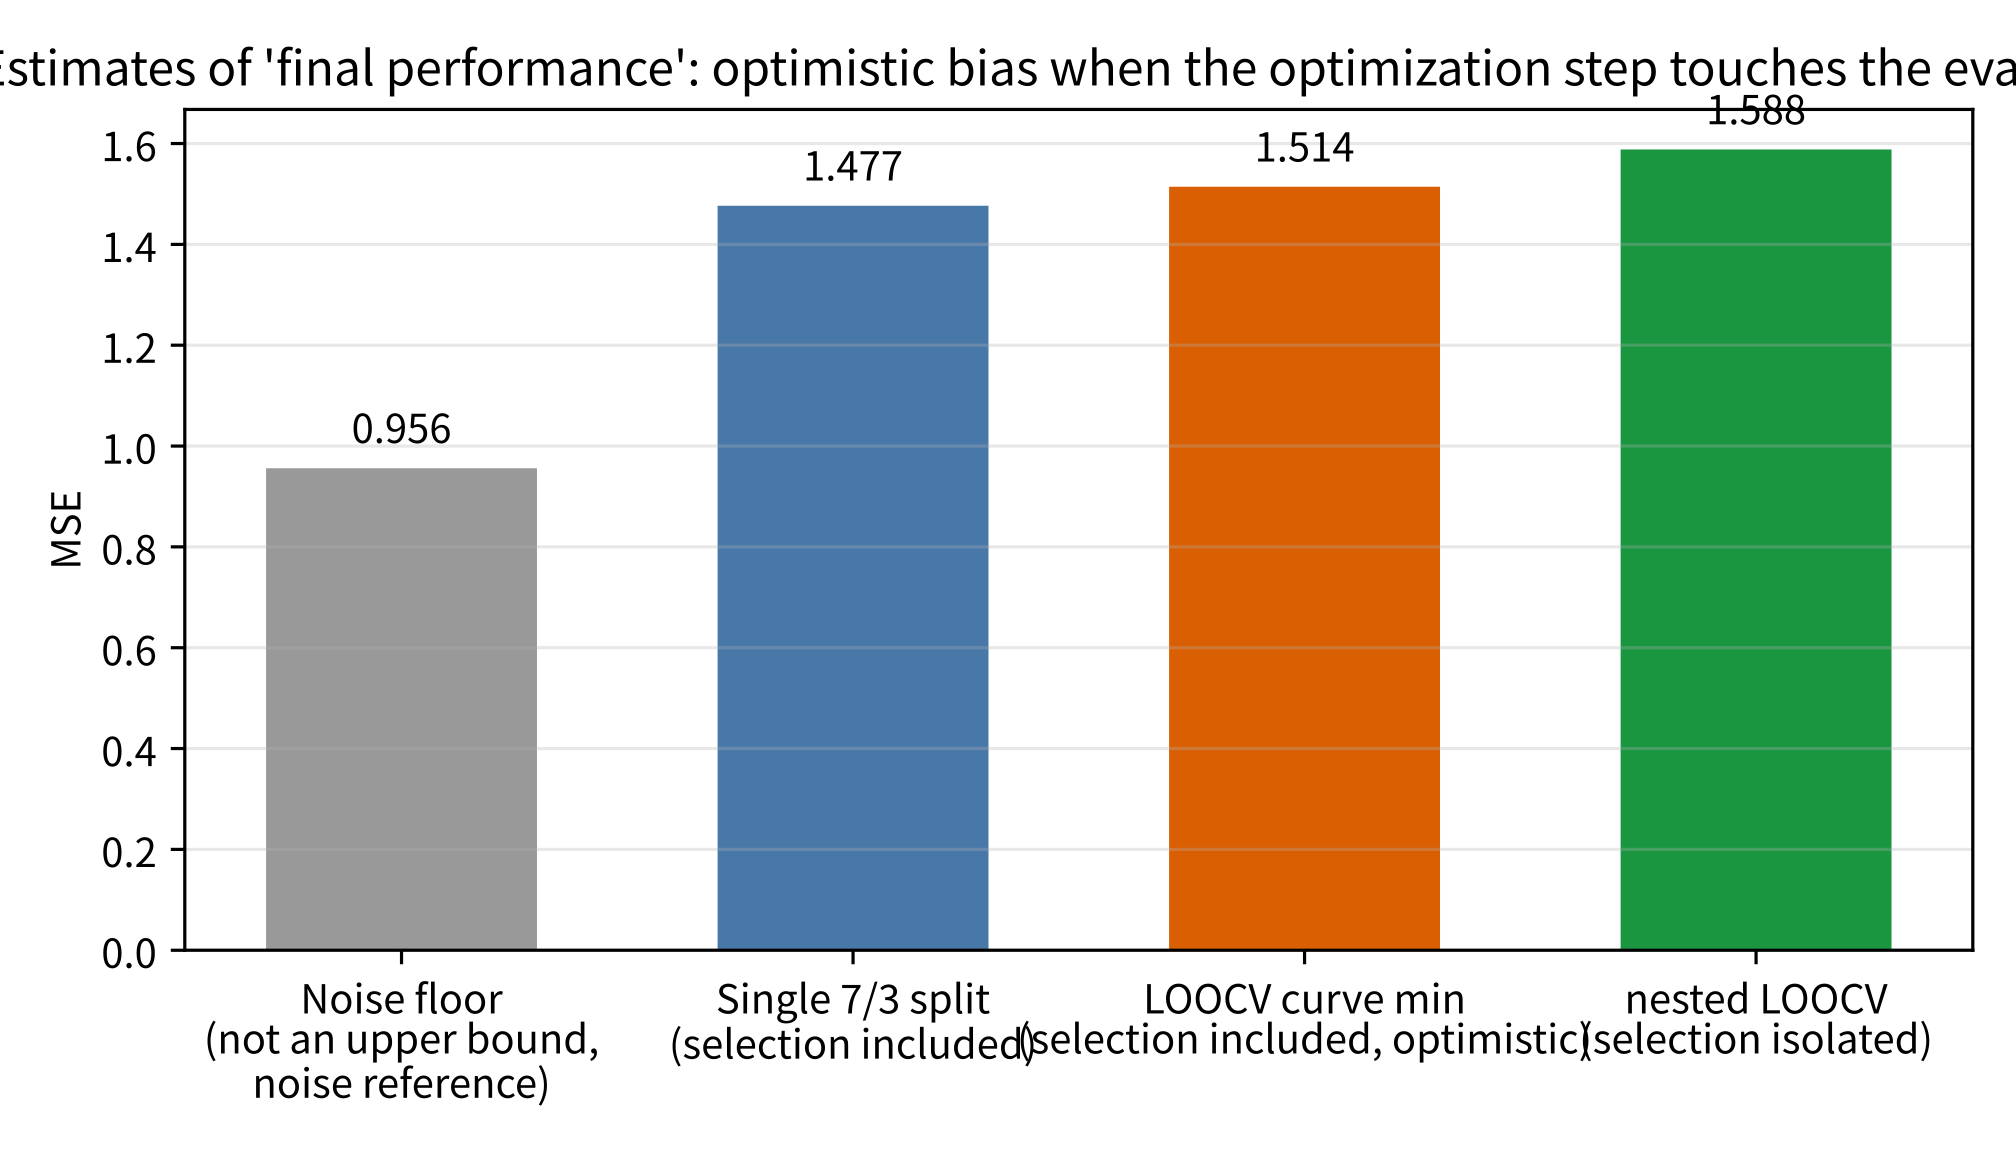
\includegraphics[width=0.54\linewidth]{ch06_2_nested_cv.png}
  \end{center}
  {\footnotesize 외층 fold: 검증용 점 1개(녹색). 내층: 남은 데이터로
  k-fold를 돌려 $\lambda$ 선택(주황 박스, ``선택은 여기에서만'').
  정보 흐름이 외층 검증 데이터에 닿지 않도록 내층 $\to$ 외층 방향으로만.}
  \vskip0.4em
  \begin{itemize}
    \item 원칙적인 고치: 데이터를 \textbf{두 층으로 분리}.
    \item \emph{외층} 검증 데이터는 ``최종 측정''에만, $\lambda$를 고르는
      \emph{모든} 선택 단계는 \emph{내층}에서만.
  \end{itemize}
\end{frame}

\begin{frame}{편향이 실제로 얼마인지: 숫자로}
  ($m=10$, 특징 1개, $\lambda\in\{0,1,10\}$)
  \small
  \begin{tabular}{@{}p{4.4cm}rl@{}}
    \toprule
    추정 방법 & 추정 MSE & 선택이 평가에 닿는가 \\
    \midrule
    노이즈 플로어(참고선) & 0.956 & --- \\
    (a) 단일 7/3 분할 & 1.477 & 평가 3개에는 안 닿음 \\
    (b) LOOCV 곡선의 min & \textbf{1.514} & \textbf{당함} — 곡선 전체가 10개로 그림 \\
    (c) nested LOOCV & 1.588 & 안 닿음(선택은 전부 내층 9개) \\
    \bottomrule
  \end{tabular}
  \par\vskip0.5em\normalsize
  \kq{핵심은 (b) vs (c): (c)가 (b)보다 \textbf{0.07} 높게 — 이 갭이
  ``곡선 최소점을 최종 성능으로 보고한'' 것에 배어 있던 낙관적 편향.}
  \vskip0.3em
  \begin{itemize}
    \item (c)의 내부 선택: 10번 중 9번 $\lambda=1.0$, 1번 $\lambda=0.0$ —
      선택이 \emph{데이터에 따라서} 흔들리는 것 자체가 §1SE 규칙의 경고.
    \item $m=10$·후보 3개라 갭이 작지만 구조는 6.3과 동일 — 후보 100개,
      $\sigma=1$이면 $\mathbb{E}[\max]\approx2.5$까지 부풀어
      \textbf{후보 수·흔들림이 커질수록 갭도 함께 커진다}.
  \end{itemize}
\end{frame}

\begin{frame}{실전 가이드라인: ``항상 nested CV''가 아니다}
  nested CV는 보통 CV보다 $k$배 가까운 학습 횟수를 먹는다.
  \begin{itemize}
    \item 보통 CV로 $\lambda$를 \textbf{고르는 것}(selection)은 당연 —
      그것이 val의 정당한 용도.
    \item \textbf{보고(reporting)}할 때는, 어떤 선택에도 쓰인 적 없는
      \textbf{홀드아웃 데이터}(6.3의 test set)로 재는 것이 원칙.
    \item 홀드아웃이 없는 상황(경진대회, 데이터 전부 소진)이라면 nested CV가
      ``같은 데이터로 정직한 추정치를 얻는'' 방법.
  \end{itemize}
  \vskip0.5em
  \begin{block}{이 절의 $\lambda$ 선택이 만드는 최적화 편향}
    ``어떤 데이터로 무엇을 고르고, 어떤 데이터로 최종 측정하는가''를
    엄격한 원리로 정리하는 것이 바로 6.3의 주제.
  \end{block}
\end{frame}

\begin{frame}{자주 묻는 질문 (1)}
  \textbf{Q. $k$는 몇으로?}
  \begin{itemize}
    \item $k=5$ 또는 $10$이 실전 기본값.
    \item $k$가 클수록($k=m$, \kb{LOOCV}) 각 fold 학습 데이터가 거의 전체 →
      편향 줄지만, fold를 $m$번 다시 학습 → 비용↑ · fold 간 분산↑.
    \item $k$가 작을수록($k=3$)은 빠르지만 fold 학습 데이터 작아 편향↑.
    \item $5\sim10$이 실용적 절충점.
  \end{itemize}
  \vskip0.4em
  \textbf{Q. 교차검증은 항상 해야 하나요?}
  \begin{itemize}
    \item 데이터가 아주 많으면(수백만 개) 한 번만 train/val로 나눠도 검증셋이
      충분히 커 안정적인 평가.
    \item 적을수록(수백$\sim$수천) 한 번의 분할이 우연히 ``쉬운/어려운''
      검증셋을 뽑을 위험이 커 → 교차검증의 가치↑.
  \end{itemize}
\end{frame}

\begin{frame}{자주 묻는 질문 (2)}
  \textbf{Q. 경진대회(Kaggle)에서 test 라벨이 안 공개되면?}
  \begin{itemize}
    \item 공개 \kb{public leaderboard}는 사실상 \emph{val}, 비공개
      \kb{private}는 \emph{test} 역할.
    \item public 점수로 $\lambda$를 골라 계속 제출하면, public을
      ``20번 봤다''는 뜻 → §최적화 편향 관점에서 public 점수는
      \textbf{부풀려진} 추정치. private의 제출 횟수 제한이 바로 이
      선택 편향을 통제하기 위함.
    \item \kq{교훈: 같은 검증 조각으로 비교한 후보가 $m$개면, 그 검증
      점수는 $m$개 중 max를 본 셈.}
  \end{itemize}
  \vskip0.4em
  \textbf{Q. k-fold CV 평균은 ``진짜 성능''의 공정한(무편향) 추정치?}
  \begin{itemize}
    \item ``한 모델 평가'' 용도라면 같은 분포의 새 데이터 기대 오차에 대한
      합리적 추정치.
    \item ``여러 $\lambda$ 후보 중 \emph{최솟값}을 고르는'' 용도로 쓰면
      그 최솟값은 평균적으로 \emph{낮게}(낙관적) — 정직한 숫자가 필요하면
      선택에 쓰지 않은 test(6.3)나 nested CV를 쓴다.
  \end{itemize}
\end{frame}

\begin{frame}{확인 문제 6.2}
  \small
  \begin{enumerate}
    \item 샘플 10개(인덱스 0$\sim$9)를 $k=5$로 \texttt{k\_fold\_split}.
      \texttt{fold\_idx=2}일 때 val에 들어가는 인덱스를 쓰고, 5개 fold를
      모두 돌렸을 때 각 인덱스가 val에 총 몇 번 등장하는지 확인.
    \item 평균모델 예($y=1,\dots,10$, 순서 2개씩 5등분)에서 fold 0과 4의
      fold별 MSE를 각각 계산하고 5-fold 평균을 구해, 정직한 8.25와 CV 12.75의
      차이를 한 문장으로 설명.
    \item 아래 $\lambda$ 5개에 대한 5-fold 평균 MSE: (가) 최소점은? (나)
      최소점 $\lambda=1.0$의 fold별 MSE $=[4.2,4.4,4.6,4.8,5.0]$일 때
      1SE 규칙(최소점 평균 + fold 표준편차 1개 이내인 후보 중 \textbf{가장
      큰} $\lambda$)으로 고를 $\lambda$는?
      \newline\newline
      {\footnotesize $[\lambda: 0.1\ 0.3\ 1.0\ 3.0\ 10.0]$ /
      $[\text{MSE}: 5.00\ 4.80\ \textbf{4.60}\ 4.70\ 5.20]$}
    \item $\lambda$ 후보 20개 CV의 최소점(MSE 3.12)을 ``배포 모델의 기대
      성능''으로 보고했다. 이 주장이 왜 낙관 편향이 있는지 §최적화 편향의
      구조로 설명하고, 정직한 추정치를 얻는 두 방법(하나는 \emph{데이터}를,
      하나는 \emph{계산}을 더 요구)을 쓰라.
  \end{enumerate}
\end{frame}

\begin{frame}{6.2 정리}
  이 절은 두 가지를 손에 넣었다.
  \begin{enumerate}
    \item \textbf{절차} — k-fold CV로 전체를 ``한 번씩은 검증에도'' 쓰면서,
      학습 손실이 아니라 \emph{검증} 손실이 가장 작은 $\lambda$를 고른다:
      U자형 곡선은 6.1의 편향-분산이 실제 숫자로 그려진 것이고,
      1SE 규칙은 ``최소점'' 단일 수치에 대한 건강한 불신을 \textbf{제도화}한 것.
    \item \textbf{경고} — ``여러 후보 중 최솟값을 고르는'' 행위 자체가
      또 하나의 선택이므로, CV 곡선의 최소점은 곧바로 ``최종 성능''이 될
      수 없다.
  \end{enumerate}
  \vskip0.5em
  \kq{낙관적 편향을 격리하는 방법 — 선택에 쓰지 않은 test, 또는 nested CV —
  은 6.3의 train/val/test 분리 원리가 이 절과 맞닿는 지점.}
\end{frame}

% =====================================================================
\section{6.3 train/val/test 분리 원칙 실전}

\begin{frame}{왜 3분할이 필요한가: 배우다와 재다를 나누어야}
  머신러닝 파이프라인은 \textbf{두 가지 완전히 다른 일}을 동시에 한다:
  \begin{columns}[T]
    \begin{column}{0.5\textwidth}
      \kb{배우는 일}
      train 데이터로 모델의 파라미터를 정하는 것.
    \end{column}
    \begin{column}{0.5\textwidth}
      \kb{재는 일}
      그 모델이 \emph{보지 못한} 데이터에서 얼마나 잘하는지 평가.
    \end{column}
  \end{columns}
  \vskip0.5em
  \begin{block}{이 둘을 같은 데이터로 하면}
    모델이 ``재는 데이터''까지 보고 만들어졌으므로, 그 점수는
    ``학습을 얼마나 잘했는가''가 아니라 \textbf{``기억을 얼마나
    잘했는가''}를 재게 된다. 4.1의 과적합(``train에서 완벽, test에서
    참사'')과 \textbf{정확히 같은 구조}.
  \end{block}
  \vskip0.3em
  6.1의 정규화($\lambda$)와 6.2의 교차검증은 이 문제를 \emph{완화}했지만
  \textbf{역할 분리} 자체를 정한 곳은 아직 없다.
\end{frame}

\begin{frame}{역할 분리: 각 조각이 딱 한 역할만}
  데이터를 세 조각으로 나눠, 각 조각이 서로 다른 질문에 답하도록
  \textbf{각각 딱 한 역할만} 쓰기로 약속:
  \begin{itemize}
    \item \kb{train}은 \textbf{배운다} — 학습 데이터로 파라미터($w$)를 정.
    \item \kb{val}은 \textbf{모델을 고른다} — 하이퍼파라미터
      ($\lambda$, kNN의 $k$, 트리 깊이 등)를 정.
    \item \kb{test}는 \textbf{딱 한 번}만 최종 점수를 준다.
  \end{itemize}
  \vskip0.4em
  \begin{block}{한 줄 압축}
    \kq{``정보의 흐름 방향을 정한다''.}
    train은 val·test로, val은 최종 모델로 정보가 흐를 수 있지만,
    \textbf{test에서는 어디로도 정보가 흘러나와서는 안 된다}.
    test는 파이프라인의 \emph{마지막 관문} — 한 번 지나가면 돌아올 수 없다.
  \end{block}
  \vskip0.2em
  {\footnotesize 테스트를 하이퍼파라미터 튜닝에 쓰면 ``부정행위''
  (test를 몰래 봐서 고른 모델)와 다를 게 없다.}
\end{frame}

\begin{frame}{정보 흐름 다이어그램}
  \begin{center}
    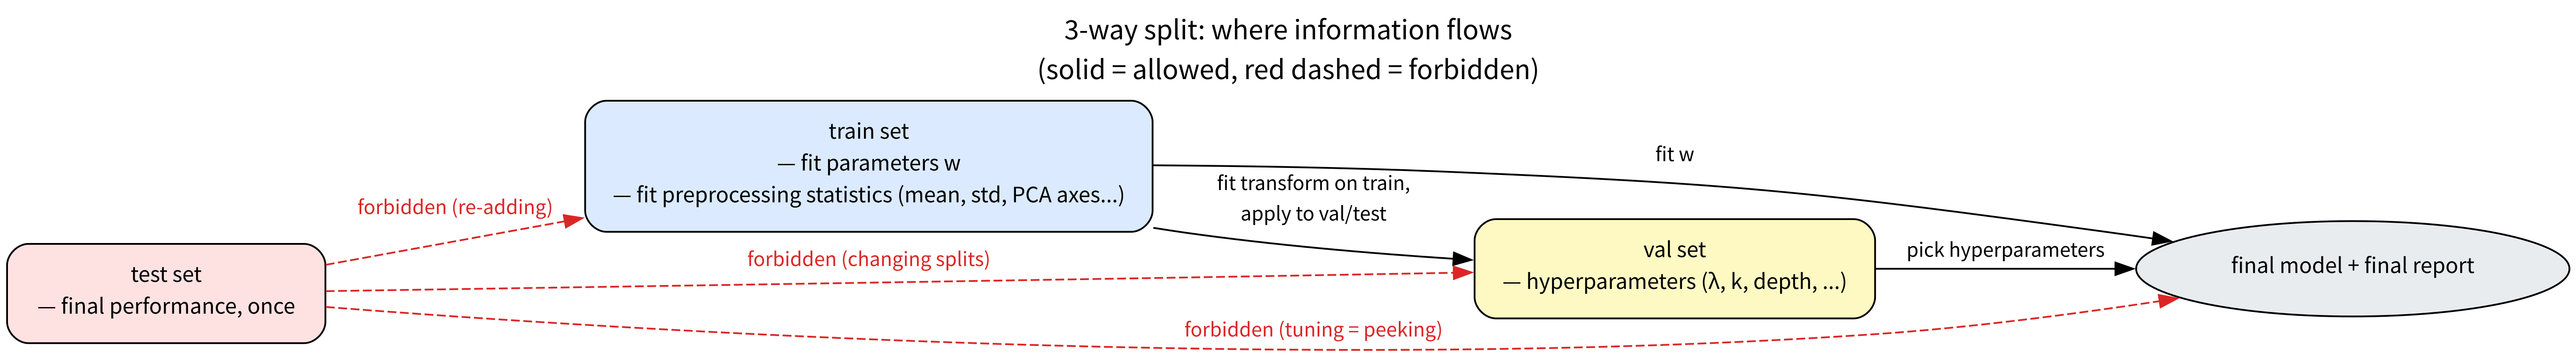
\includegraphics[width=0.52\linewidth]{ch06_3_info_flow.png}
  \end{center}
  {\footnotesize 허용된 흐름(실선)은 train에서 시작해 val을 거쳐 최종 모델로
  흐르고, \textbf{테스트(빨간 점선)에서 나가는 모든 화살표는 금지}.}
  \vskip0.4em
  \begin{itemize}
    \item \kb{train $\to$ val / test}: 전처리 통계량(평균·표준편차, PCA 축)을
      \emph{train으로만 fit}하고 val·test에는 \emph{apply} — 허용되는 유일한
      교차.
    \item \kb{train $\to$ 모델}: $w$를 fit. \quad
      \kb{val $\to$ 모델}: 하이퍼파라미터를 고르는 방향.
    \item \kb{test $\to$ (val / train / 모델)}: \textbf{모두 금지} — 전부
      ``테스트를 살짝 훔쳐보았다''는 뜻.
  \end{itemize}
  \vskip0.2em
  {\footnotesize 이 다이어그램이 이 절의 \textbf{지도}. 다음 세 절(선택
  편향, 시계열, 그룹 분할)은 이 지도의 \emph{빨간 점선을 밟아봤을 때}
  실제 숫자가 어떻게 변하는지를 보여준다.}
\end{frame}

\begin{frame}{3분할이 실제로 깨지는 흔한 실수 세 가지}
  \begin{enumerate}
    \item \kb{테스트로 여러 모델을 비교}해 가장 잘 나온 걸 고르는 것
      (``살짝 훔쳐보기'').
    \item \kb{검증 데이터 없이} 테스트 데이터로 하이퍼파라미터까지 같이
      튜닝(검증과 테스트를 사실상 섞어버림).
    \item 데이터를 나누기 \textbf{전에} 정규화(스케일링) 같은 전처리
      통계량(평균, 표준편차)을 \textbf{전체 데이터}로 계산 — test 정보가
      전처리 단계에서 이미 학습에 스며듦(\kb{data leakage}).
  \end{enumerate}
  \vskip0.4em
  세 실수가 모두 같은 범주 — \textbf{``test 정보가 다른 곳으로 흘러나감''} —
  에 속한다. 겉모양은 달라(모델 고르기 / 전처리 순서 / …) 보여도
  \textbf{다 같은 정보 흐름의 역주행}.
  \vskip0.3em
  \begin{block}{더 좋은 질문}
    ``이 코드에 leakage가 있는가?''보다:
    \kq{``test(또는 val)의 정보가 학습이나 선택 단계에 닿았는가?''}
    \vskip0.2em
    아래 §에서 이 질문을 \textbf{숫자로} 답할 수 있는 도구를 하나씩 만든다.
  \end{block}
  {\footnotesize Ch.\,8, 16 팀 프로젝트와 ML2에서도 이 3분할 원칙을 그대로
  지켜야 한다.}
\end{frame}

\begin{frame}{손으로 한 번: 누수를 숫자로}
  세 번째 실수(정규화 통계량을 전체 데이터로 미리 계산)가 어떤 왜곡을
  만드는지. 값 $1\sim10$을 앞 7개(train)·뒤 3개(test)로 나눔:
  \small
  \begin{tabular}{@{}lcc@{}}
    \toprule
    기준 & 평균 & 표준편차 \\
    \midrule
    전체 10개(누수) & 5.5 & 2.872 \\
    train 7개만(올바름) & 4.0 & 2.000 \\
    \bottomrule
  \end{tabular}
  \par\vskip0.5em\normalsize
  test $=[8,9,10]$를 각각의 통계량으로 표준화:
  \[
  \text{전체(누수)}: [0.870,\ 1.219,\ 1.567]\qquad
  \text{train(올바름)}: [2.0,\ 2.5,\ 3.0]
  \]
  \begin{itemize}
    \item 전체 데이터로 미리 계산한 평균·std를 쓰면 test 값이 실제보다
      훨씬 ``평범(z값 작음)''해 보인다 — std 자체가 test의 큰 값들 때문에
      이미 커져 있기 때문(2.872 vs 2.0).
  \end{itemize}
\end{frame}

\begin{frame}{배포 시나리오: 미래를 볼 수 없다}
  \begin{itemize}
    \item 모델을 배포하는 시점에는 \textbf{미래에 들어올 데이터(test에
      해당)를 아직 볼 수 없음} → 애초에 그 통계량을 계산에 쓸 수 없다.
    \item \kb{train 통계량만으로 표준화}가 실제 배포 상황을 정확히 흉내
      낸 것이고, 전체 데이터로 계산하는 것은 ``미래를 몰래 들여다본'' 값.
    \item 이 차이가 검증 성능을 \textbf{실제보다 낙관적으로 부풀리는}
      방향으로 작용하는 경우가 많다.
  \end{itemize}
  \vskip0.4em
  \begin{center}
    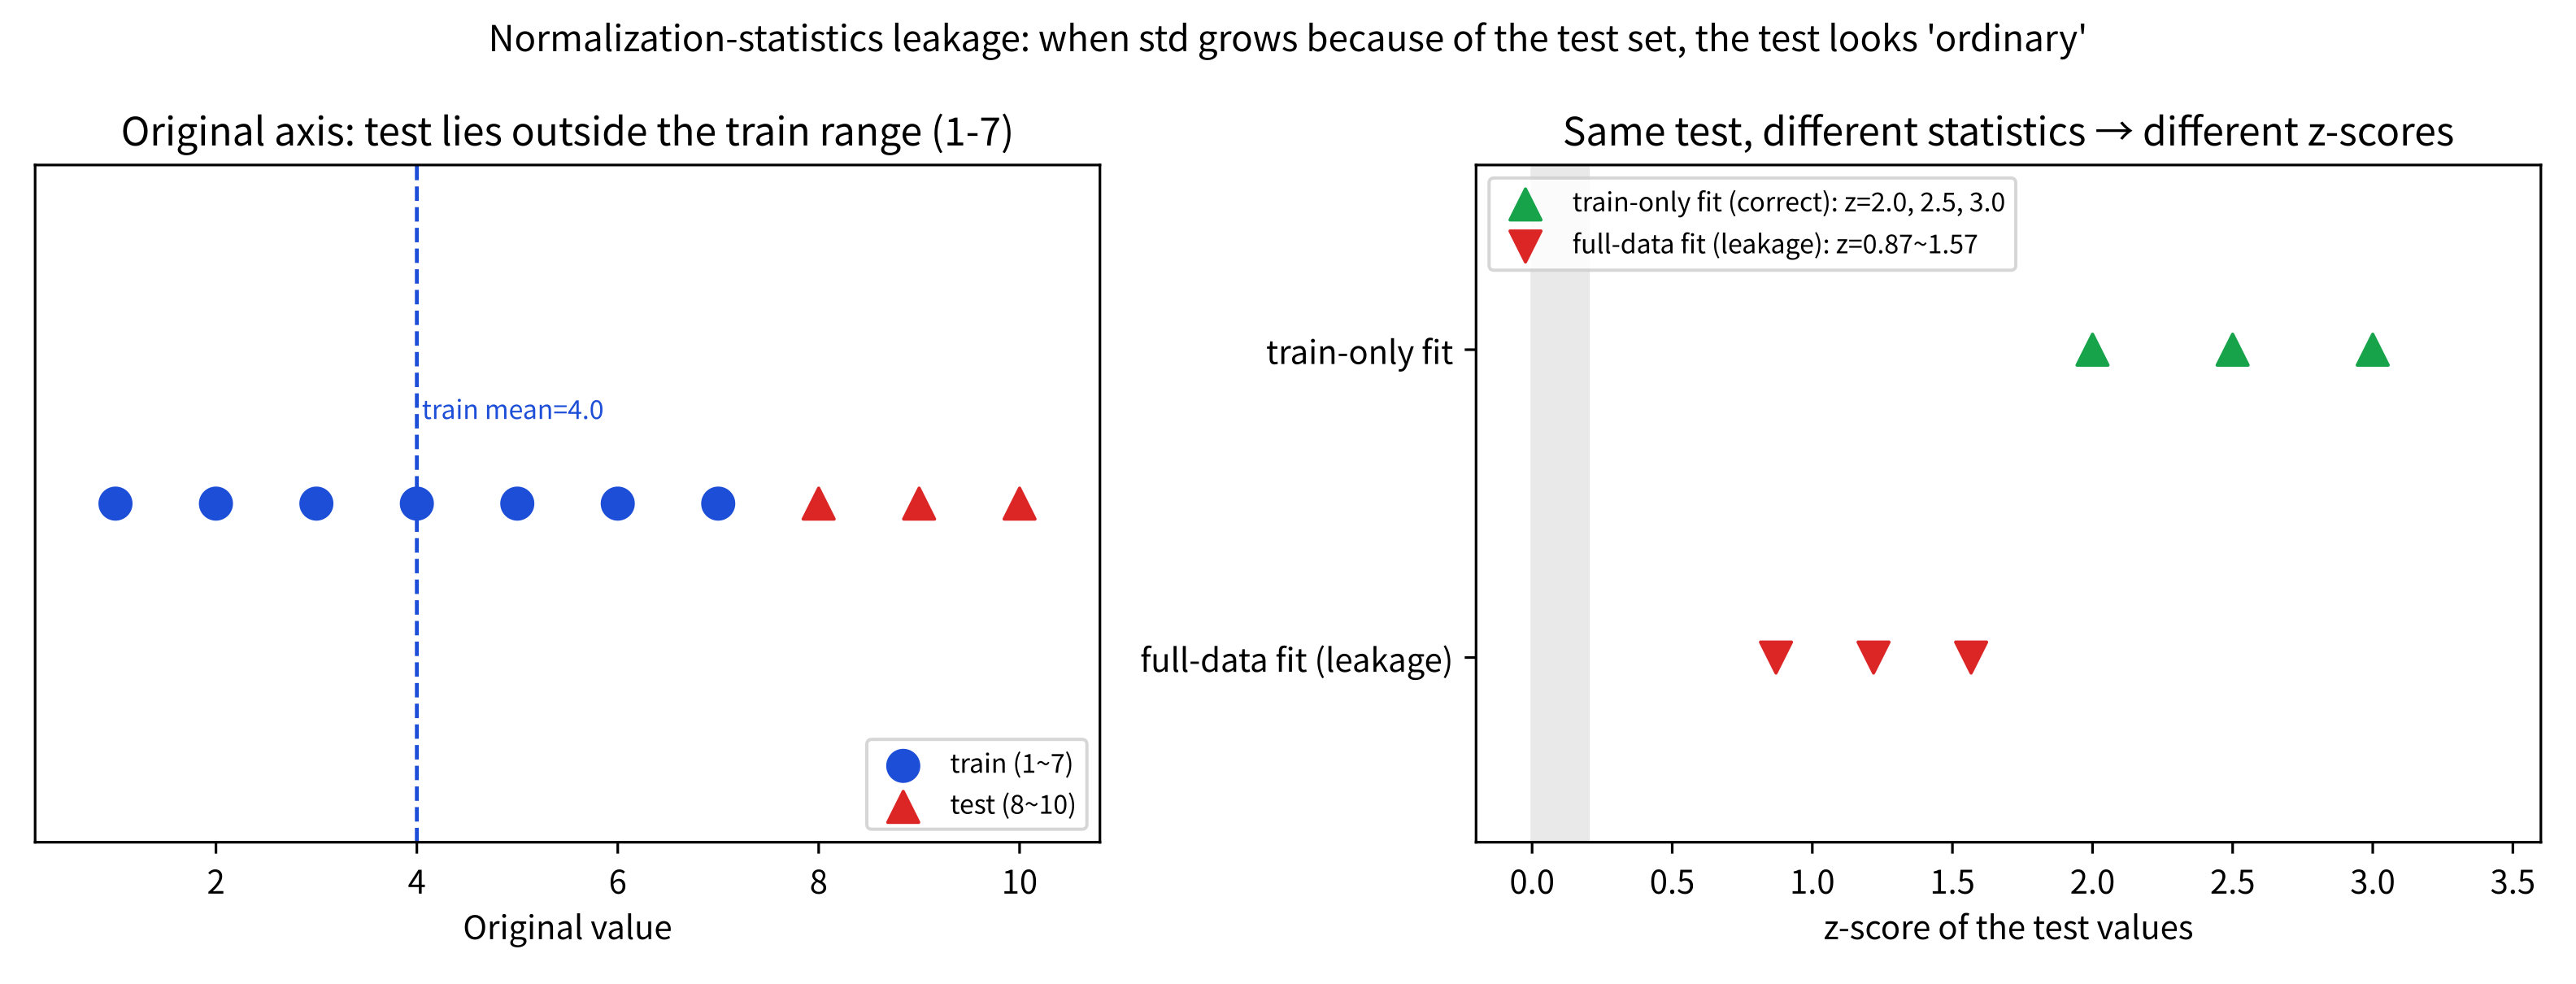
\includegraphics[width=0.5\linewidth]{ch06_3_leakage_zscore.png}
  \end{center}
  {\footnotesize 좌측: 원본 축에서 test(8$\sim$10)는 train 범위(1$\sim$7)를
  벗어남. 우측: 전체로 fit한 std(2.87)로 나누면 test의 z가 0.87$\sim$1.57로
  ``평범'', train만 fit한 std(2.0)로 나누면 2.0$\sim$3.0으로 ``극단''.}
  \vskip0.3em
  \begin{block}{왜 std가 test 때문에 커지는가}
    전체 10개의 std(2.872)가 train 7개(2.0)보다 큰 것은, test의 큰 값들
    (8,9,10)이 \emph{분산 계산에 이미 들어와} 전체 std를 끌어올린 것.
    \vskip0.2em
    \kq{재고 싶은 것(test)이 재는 자(통계량)를 미리 바꿔놓은 것 = 누수의
    핵심.}
  \end{block}
  {\footnotesize PCA(Ch.\,14)의 주성분, 결측치 대체 평균 등 ``데이터를 보고
  계산하는 \emph{모든} 통계량''에 동일 — \textbf{반드시 train으로만 계산하고,
  val/test에는 적용만}.}
\end{frame}

\begin{frame}[fragile]{scikit-learn의 표준 구현}
\begin{lstlisting}
# 올바른 순서: train으로만 fit, val/test에는 transform만
scaler = StandardScaler().fit(X_train)
X_val  = scaler.transform(X_val)
X_test = scaler.transform(X_test)
\end{lstlisting}
  {\footnotesize \texttt{.fit\_transform(X\_all)}을 val·test에 쓰면
  ``누수'' 열과 동일한 위장이 일어난다.}
\end{frame}

\begin{frame}{``살짝 훔쳐보기''의 통계: 선택 편향}
  ``테스트로 여러 후보를 돌려보고 제일 잘 나온 걸 고른다'' — 이 한 줄이
  \emph{정량적으로} 얼마나 낙관적인지 확률로 계산.
  \begin{itemize}
    \item 각 후보의 테스트 성능을 (진짜 성능 + 우연한 잡음)으로 모델링,
      잡음을 독립 정규분포 $\mathcal{N}(0, \sigma^2)$.
    \item 후보 $m$개 중 \textbf{최고 점}을 고르는 행위 = $m$번의 잡음
      뽑기 중 $\max$를 고르는 것과 같음.
    \item $m$개 독립 정규분포의 $\max$는 평균(=0, 진짜 성능)보다
      \textbf{항상 위쪽으로 치우침} — $m$이 커질수록 max는 더 위로.
  \end{itemize}
  \vskip0.4em
  {\footnotesize 이 편향을 정량화한 대표 논문: Varma·Simon (2006).}
\end{frame}

\begin{frame}{$\mathbb{E}[\max]$를 숫자로}
  $\sigma=1$, 진짜 성능 0인 경우 4만 번 시뮬레이션. 후보 수 $m$에 따른
  ``고른 최고 점''의 평균:
  \small
  \begin{tabular}{@{}cccccccc@{}}
    \toprule
    $m$ & 1 & 2 & 5 & 10 & 20 & 50 & 100 & 500 \\
    \midrule
    $\mathbb{E}[\max]$ & $\approx0$ & 0.56 & 1.16 & 1.53 & 1.86 & 2.25 & 2.51 & 3.04 \\
    \bottomrule
  \end{tabular}
  \par\vskip0.4em\normalsize
  \begin{center}
    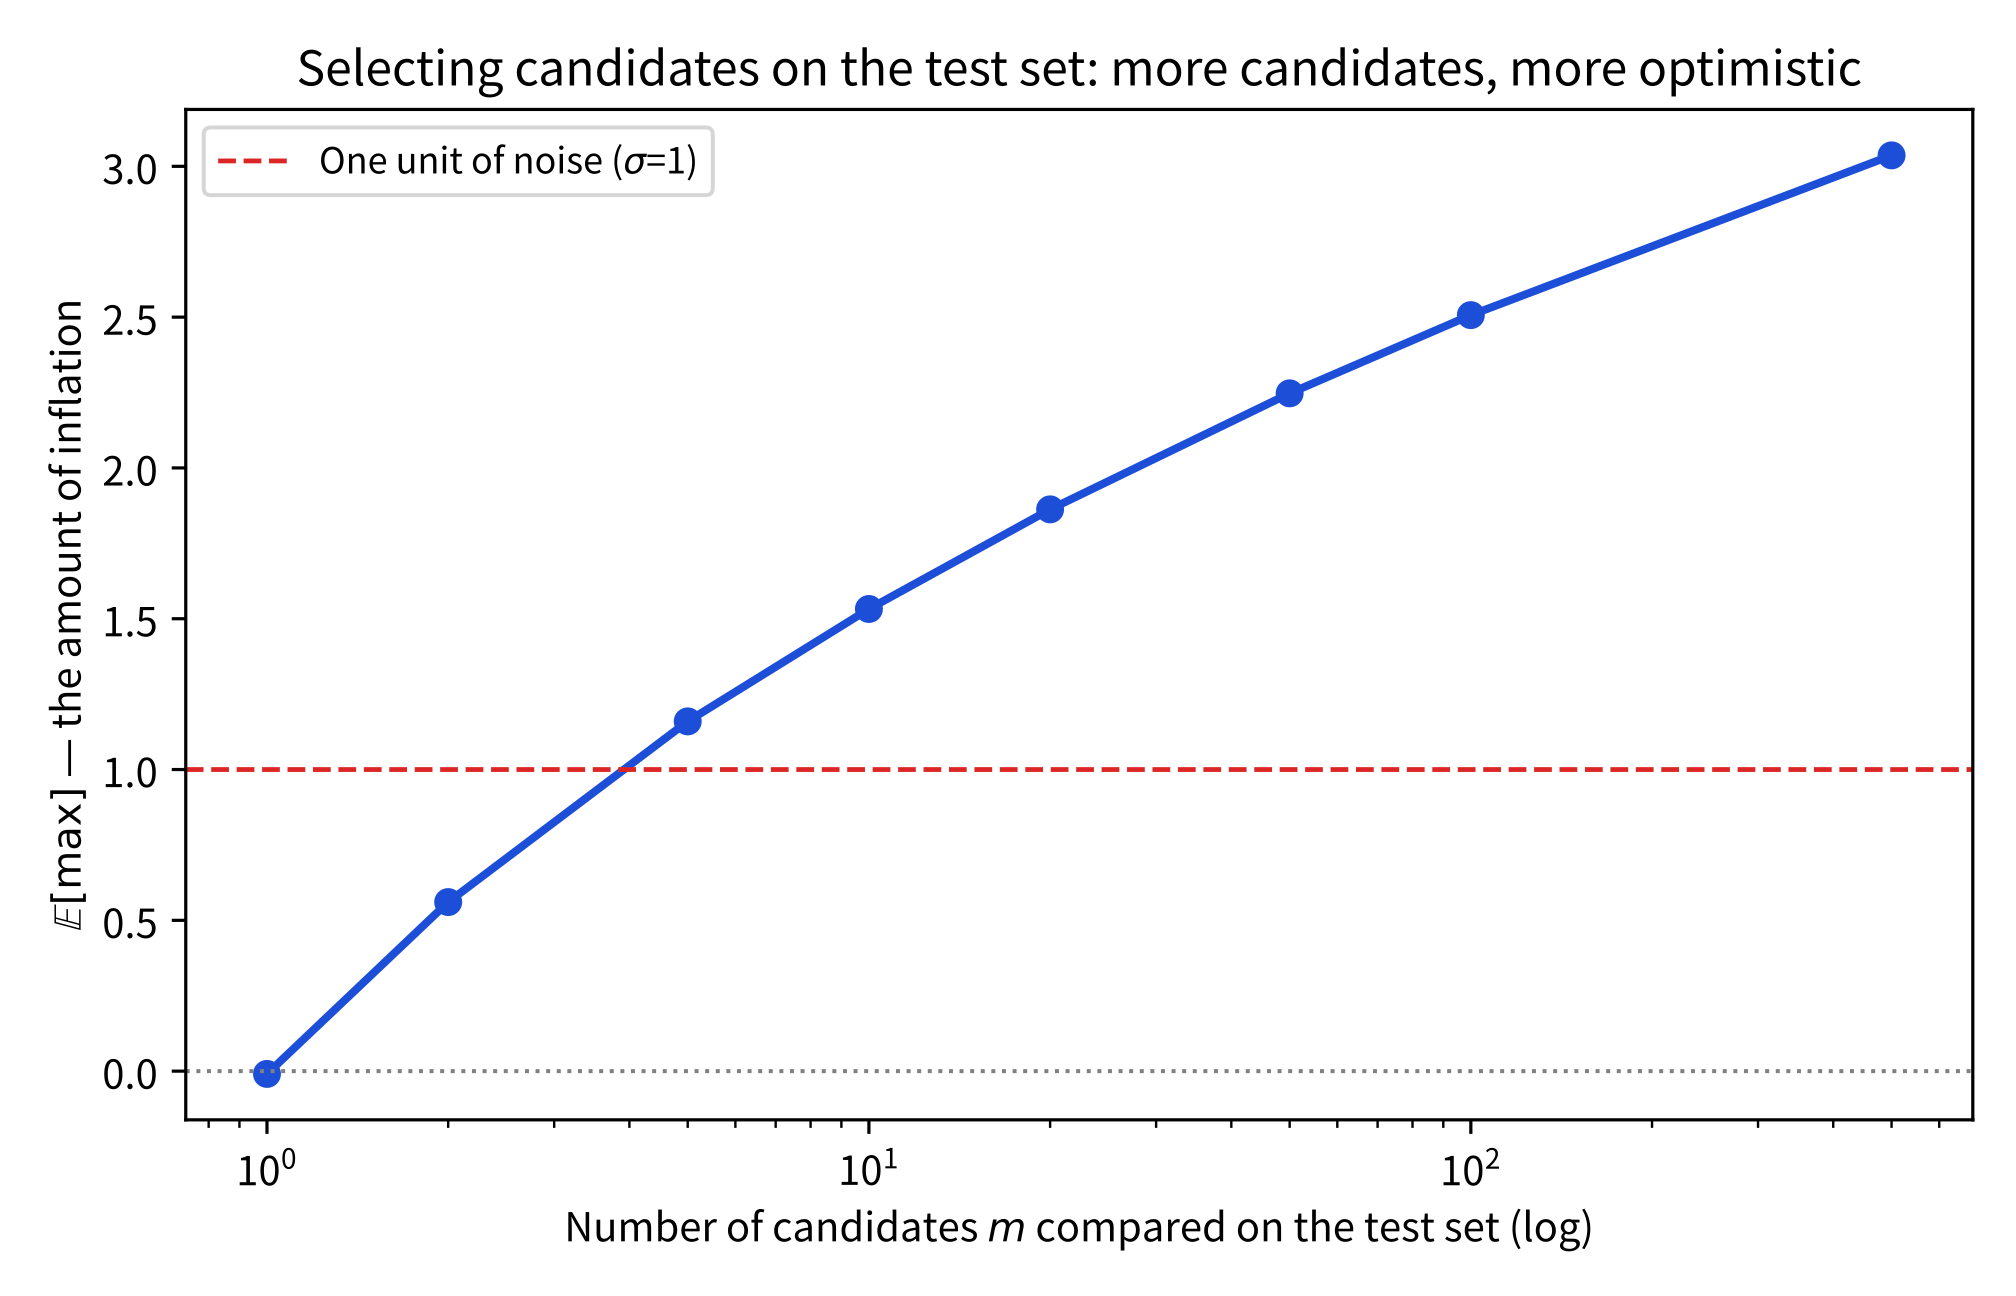
\includegraphics[width=0.46\linewidth]{ch06_3_selection_bias.png}
  \end{center}
  {\footnotesize 후보 수 $m$(로그 축)에 따른 $\mathbb{E}[\max]$ — 잡음 한
  개($\sigma=1$)를 붉은 점선으로. $m=50$이면 잡음의 2배 이상, $m=100$이면
  2.5배 부풀어 오름.}
  \vskip0.3em
  \begin{itemize}
    \item $m=1$이면 편향 0 — 후보 한 개면 ``고르다''는 행위가 없음.
    \item $m=5$만 되도 $\approx1.16$, $m=50$이면 $\approx2.25$ —
      \textbf{잡음 한 개의 2배 이상}이 부풀려 올라감.
    \item 실전 $m$은 ``모델 수 $\times$ 하이퍼파라미터 수''의 \textbf{곱}으로
      커지기 쉬움(모델 5개 $\times$ $\lambda$ 20개 = 100개 → 부풀림
      $\approx2.5$). 후보가 쌓이면 편향은 \emph{로그 스케일로} 계속 커짐.
  \end{itemize}
\end{frame}

\begin{frame}{val에 걸리는 편향은 정직하다}
  \begin{itemize}
    \item 이 편향이 \textbf{test가 아니라 val에 걸리는 한} 정직 — val은
      ``모델을 고르는 역할''이라 선택 편향을 \emph{예상대로} 먹고.
    \item \textbf{test는 한 번만 마지막에} 쓰이므로 그 편향에 노출되지
      않음.
    \item 그런데 test로 고르면 \emph{재야 할 대상(test)이 고르는 과정에
      쓰여서} test 자체가 $\mathbb{E}[\max]$를 그대로 먹음 —
      \textbf{평가자가 동시에 선수 선발위원}이 되는 셈.
  \end{itemize}
  \vskip0.4em
  {\footnotesize $\sigma$는 ``성능 측정의 흔들림'' 크기 — 실제에선 $\sigma$를
  곱하면 됨(잡음 3배면 부풀림도 3배).}
  \vskip0.3em
  \kq{한 줄 교훈: 후보가 $m$개면 ``제일 좋은 test 점''은 진짜 성능보다
  $\mathbb{E}[\max]$만큼 \emph{평균적으로} 높다. $m$이 1이어야 정직하고,
  크면 그 수치는 \emph{하한}이 아니라 \emph{낙관적 상한}에 가까움.}
\end{frame}

\begin{frame}{자주 하는 실수: 시계열을 무작위로 나누기}
  환자에게 있는 ``단위'' 문제의 다른 얼굴이 \textbf{시간 순서}.
  시계열은 \textbf{데이터가 이미 시간순 정렬되어 있을 때 무작위 shuffle이
  구조를 깨는} 방향으로 작용.
  \vskip0.3em
  \small
  추세(매일 $+1$)가 있는 일일 데이터 365일, kNN:
  \begin{tabular}{@{}ll@{}}
    \toprule
    분할 방식 & test RMSE \\
    \midrule
    무작위 분할 & 0.81 \\
    시간순 분할(뒤 20\% = test) & 44.1 \\
    \bottomrule
  \end{tabular}
  \par\vskip0.5em\normalsize
  \begin{itemize}
    \item \kb{무작위}: test 점들이 시간축 곳곳에 흩어져 각 test 점 근처에
      train 점이 항상 있음(과거든 미래든) → kNN이 잘 맞힘. 그런데
      \textbf{미래 값을 과거 값으로 ``예측''}한 것 — 실전(미래는 아직
      없음)에선 성립하지 않음.
    \item \kb{시간순}: test가 train의 시간 범위(horizon)를 벗어나 kNN이
      밖으로 외삽, 추세를 못 쫓아 RMSE 급등.
  \end{itemize}
  \vskip0.2em
  \begin{block}{교훈}
    이 \textbf{44.1이 실제 일반화 성능에 가까운 값}. 시계열은 무작위가
    아니라 \textbf{시간순으로} 나눠야 하고, 더 근본적으로
    \kq{``실전에서 겹치지 않을 것''을 같은 조각에 두지 말라}.
    {\footnotesize \texttt{train\_test\_split(shuffle=False)} /
    \texttt{TimeSeriesSplit}. 그룹(환자·기기·지점): \texttt{GroupKFold}.}
  \end{block}
\end{frame}

\begin{frame}[fragile]{실습: diabetes 3분할 파이프라인 전체}
  \small
\begin{lstlisting}
X, y = load_diabetes().data, load_diabetes().target  # 442건, 10개 특징
# 1) 2단계 3분할: 40%를 (val+test)로, 그 40%를 절반씩
Xtr, Xtemp, ytr, ytemp = train_test_split(X, y, test_size=0.4, random_state=0)
Xva, Xte, yva, yte = train_test_split(Xtemp, ytemp, test_size=0.5, random_state=0)
# 2) val RMSE로만 lambda 고르기 (선택 편향은 val에서만)
lams = [0.1, 1.0, 10.0, 100.0, 1000.0]
val_rmse = {lam: np.sqrt(mean_squared_error(
    yva, Ridge(alpha=lam).fit(Xtr, ytr).predict(Xva))) for lam in lams}
best = min(val_rmse, key=val_rmse.get)
# 3) 그 lambda로 train만 fit, test RMSE 한 번만
final = np.sqrt(mean_squared_error(
    yte, Ridge(alpha=best).fit(Xtr, ytr).predict(Xte)))
\end{lstlisting}
  (4) 대조로 (잘못) test로 $\lambda$를 고르면 어떤 차이가 나는지 본다.
\end{frame}

\begin{frame}[fragile]{실행 결과: 핵심은 숫자보다 절차}
  \small
  \begin{verbatim}
크기: train=265  val=88  test=89
val RMSE per lambda: {0.1: 58.07, 1.0: 61.75, 10.0: 73.04,
                      100.0: 77.49, 1000.0: 78.07}
val로 고른 lambda = 0.1  ->  최종 test RMSE (한 번만) = 53.79
(잘못) test로 고르면 lambda = 1.0
  \end{verbatim}
  \par\normalsize
  \begin{block}{핵심}
    val로 고른 $\lambda$와 test로 고른 $\lambda$는 (이 작은 데이터에서)
    \emph{같을 수도, 다를 수도} 있다 — 위 실행에선 0.1 vs 1.0으로 다름.
    \vskip0.2em
    우연히 같아도 \emph{원칙적으로} test를 선택에 썼으므로 그 test 수치는
    선택편향의 $\mathbb{E}[\max]$를 먹고 있는 \textbf{부풀려진 추정치}.
    \vskip0.2em
    \kq{같은 모델·같은 코드인데도 ``$\lambda$를 어디서 고르느냐''만 달라져
    최종 test 점의 \emph{신뢰성}이 달라짐 — 3분할은 ``코드가 아니라
    \emph{절차}''의 문제.}
  \end{block}
\end{frame}

\begin{frame}{2단계 3분할은 정말 겹치지 않는가}
  실전에선 \emph{한 번에} 3등분보다 \textbf{2단계}로 나눔: 전체 40%를
  (val+test)로 떼고, 그 40%를 다시 절반씩 val/test로.
  \vskip0.3em
  샘플 100개(0$\sim$99)를 ``앞 60=train, 뒤 40=temp'' 1차 분할 후
  temp(60$\sim$99)를 ``앞 20=val, 뒤 20=test'' 2차:
  \small
  \begin{tabular}{@{}lcc@{}}
    \toprule
    조각 & 인덱스 범위 & 개수 \\
    \midrule
    train & 0$\sim$59 & 60 \\
    val   & 60$\sim$79 & 20 \\
    test  & 80$\sim$99 & 20 \\
    \bottomrule
  \end{tabular}
  \par\vskip0.5em\normalsize
  \begin{itemize}
    \item 세 범위가 \textbf{서로 겹치지 않는지}(train/val, train/test,
      val/test 두루) — 교집합이 빈집합인지.
    \item val $\cup$ test가 ``처음 떼어둔 뒤 40\%''(60$\sim$99)와
      \textbf{등치}하는지.
  \end{itemize}
  {\footnotesize ``한 번에 3등분''과 ``2단계 분할''이 동일한 disjoint 조건을
  만족함을 보이면, 2단계 분할을 써도 3분할 원칙을 위반하지 않음이 확인.}
\end{frame}

\begin{frame}{유명한 사례: 환자 단위 누수}
  의료 영상 AI에서 실제로 자주 발견되는 누수 — \textbf{같은 환자의 여러 장
  스캔 중 일부는 train, 일부는 test에 무작위로 흩어지는} 경우.
  \begin{itemize}
    \item 같은 환자의 스캔은 서로 매우 비슷(같은 신체 구조, 같은 장비).
    \item 모델이 test에서 ``새로운 환자를 진단''하는 게 아니라 \textbf{``이미
      학습에서 본 그 환자를 살짝 다른 각도에서 다시 알아보는''} 셈이 됨.
    \item 논문에 보고된 정확도가 \emph{실제 새로운 환자}에게 적용했을 때보다
      \textbf{부풀려짐}.
  \end{itemize}
  \vskip0.3em
  \small
  환자 100명, 각 5장 스캔, kNN:
  \begin{tabular}{@{}ll@{}}
    \toprule
    분할 방식 & test RMSE \\
    \midrule
    무작위 분할(이미지 단위) & 1.04 \\
    환자(그룹) 분할 & 3.65 \\
    \bottomrule
  \end{tabular}
  \par\vskip0.3em\normalsize
  \begin{center}
    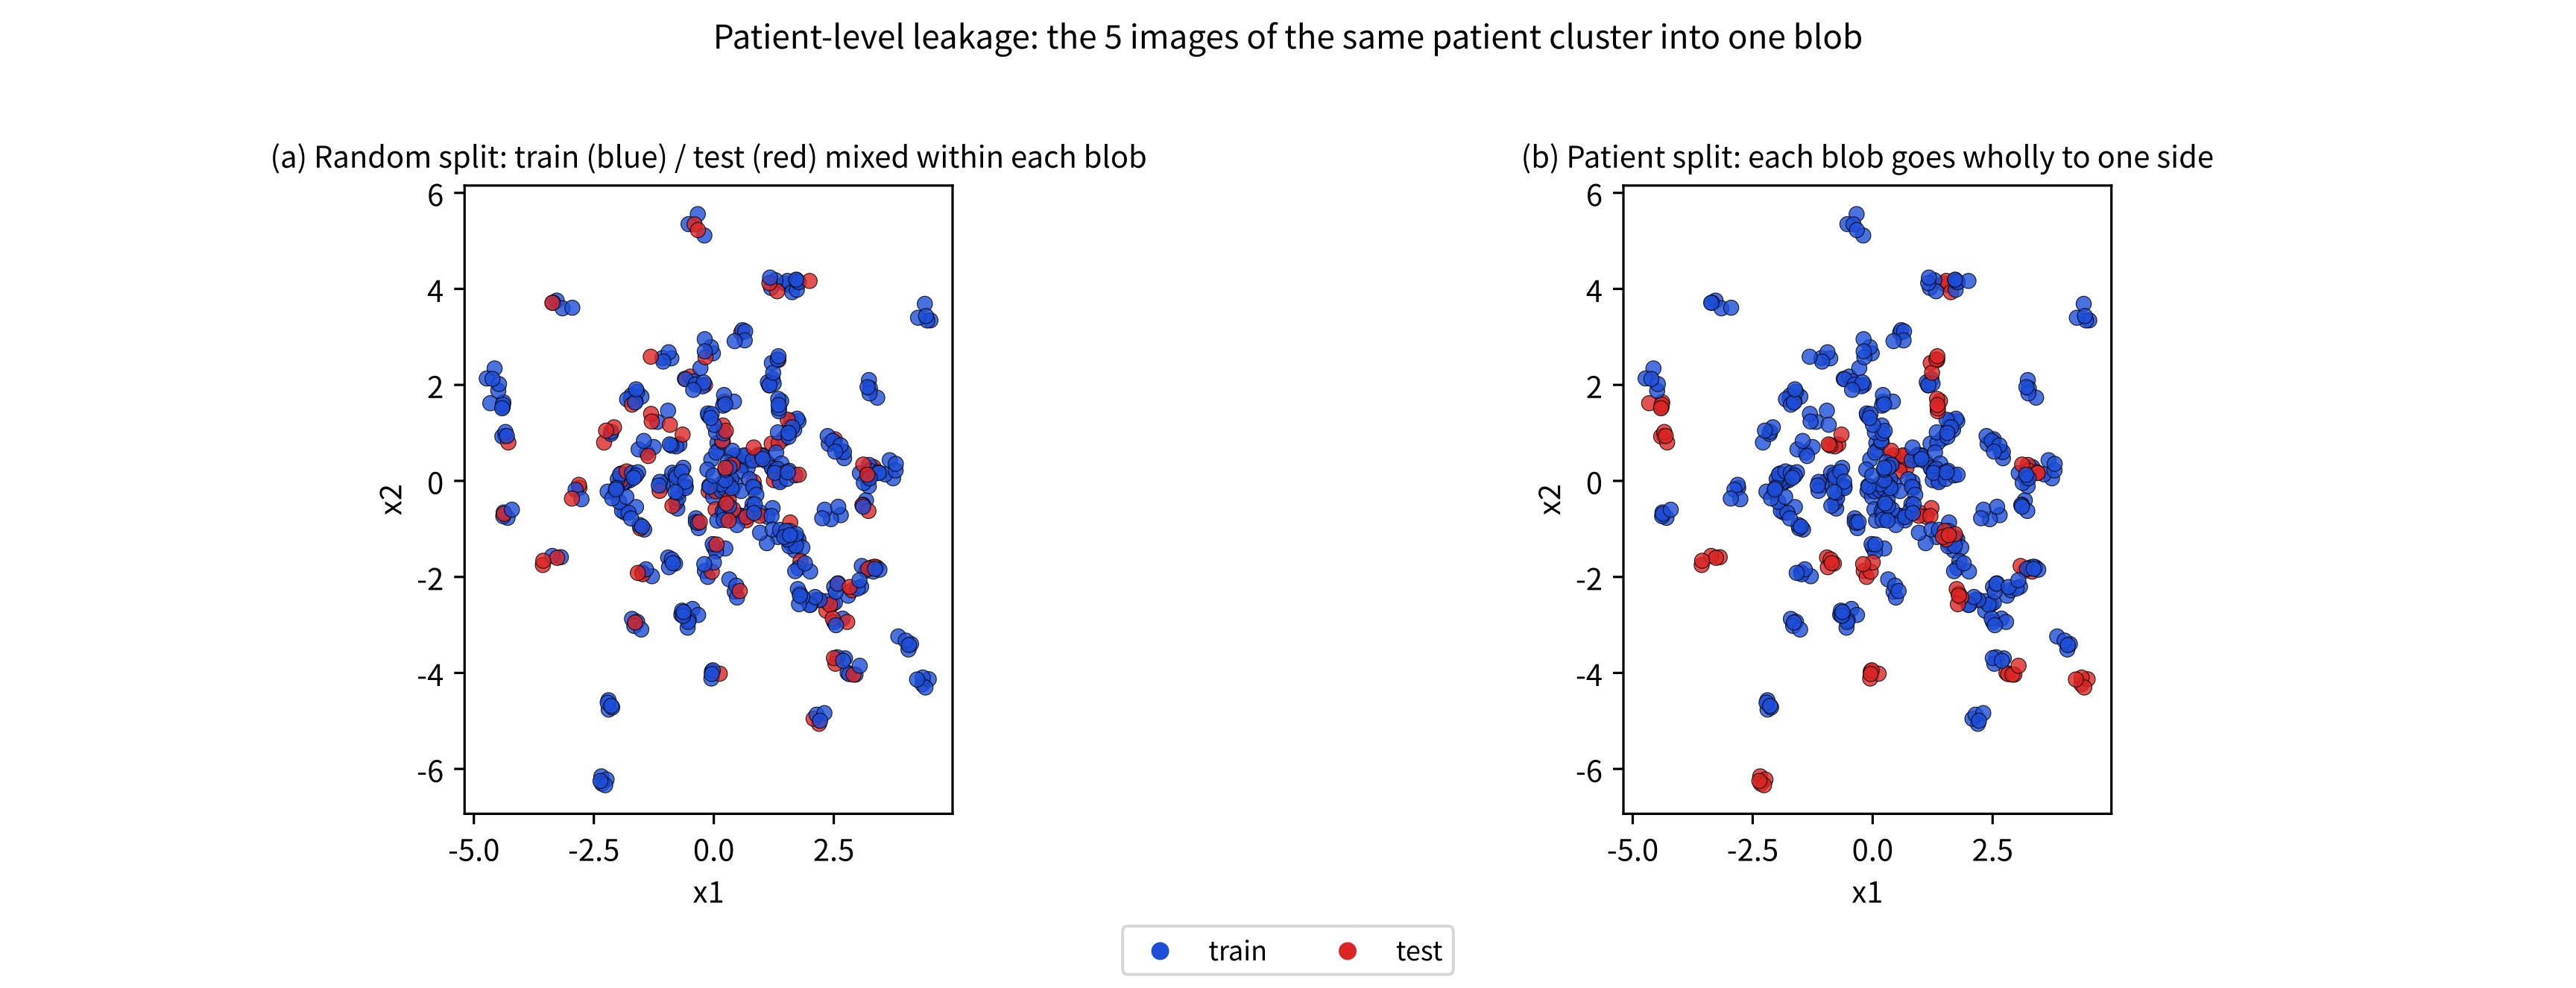
\includegraphics[width=0.44\linewidth]{ch06_3_patient_leakage.png}
  \end{center}
  {\footnotesize 이 문제는 여러 의료 AI 논문에서 사후 지적되어 재현성 논쟁으로
  이어짐(예: Rumala 2023, 뇌 MRI 종단 연구의 피험자 식별 누수).}
\end{frame}

\begin{frame}[fragile]{환자를 ``외운다'' — 왜 1.0이 ``성취''가 될 수 없는가}
  \begin{itemize}
    \item 무작위 분할 RMSE($\approx1.0$)가 환자별 값의 표준편차(2.0)보다
      \textbf{훨씬 낮음}.
    \item \kq{새로운 환자를 예측하는 것은 이론적으로
      $\sigma\sqrt{2}\approx2.8$ \emph{아래로 내려갈 수 없는데} 1.0을
      ``성취''했다.}
    \item 이건 모델이 \emph{관계를 배운} 것이 아니라 \textbf{환자를 외운
      것}.
  \end{itemize}
  \vskip0.4em
\begin{lstlisting}
from sklearn.model_selection import GroupKFold
groups = np.repeat(np.arange(100), 5)   # 100환자 x 5장, 그룹키=환자
gkf = GroupKFold(n_splits=5)
for tr_idx, te_idx in gkf.split(X, y, groups=groups):
    pass  # 같은 환자의 5장은 항상 train 또는 test 중 하나로만
\end{lstlisting}
  {\footnotesize \texttt{GroupKFold}: 각 fold마다 \emph{다른 환자}를 배정 →
  같은 환자의 5장은 \textbf{절대} train/test에 걸리지 않음. 6.2의 ``fold가
  구조를 깨면 안 된다''는 원칙의 \textbf{그룹 버전}.}
\end{frame}

\begin{frame}{자주 묻는 질문 (1)}
  \textbf{Q. 데이터가 너무 적어 3분할하면 각 조각이 너무 작아지는데?}
  \begin{itemize}
    \item test를 따로 떼는 대신, 6.2의 교차검증으로 ``학습+검증''을 반복하고,
      정말 최종 성능이 필요할 때만 별도로 확보한 \textbf{작은 test로 딱
      한 번} 확인하는 절충안.
    \item 극도로 적으면 LOOCV까지 고려. 그래도 \textbf{test를 완전히 없애고
      검증 성능만으로 최종 성능을 주장하는 것은 피해야} 한다 — 검증 성능은
      이미 하이퍼파라미터 선택에 ``간접적으로'' 쓰였기 때문.
    \item \textbf{몇 대 몇?} 정해진 정답 없음 — 60/20/20이나 70/15/15가 흔한
      시작점. 아주 많으면(수백만) val·test가 각각 1$\sim$2\%만 되어도
      안정적.
  \end{itemize}
  \vskip0.4em
  \textbf{Q. 교차검증(6.2)을 쓰면 test는 굳이 필요 없지 않나요?}
  \begin{itemize}
    \item \emph{보통}은 그렇지만, ``정확히 한 번''의 최종 성능이 필요한
      (논문 제출, 배포 전 검증) 상황에선 필요.
    \item k-fold CV는 \emph{val 역할}(하이퍼파라미터 고르기), test는
      \emph{최종 판정}(아무 선택 없이 처음 보는 데이터로 검증). CV만 있으면
      ``고르는 과정''만 있고 ``판정''이 없다.
    \item 특히 \textbf{CV를 여러 번($\lambda$마다, 시드마다) 돌리면서} test
      점수를 보고 결정 내리면, test가 다시 \emph{선택에} 쓰임.
  \end{itemize}
\end{frame}

\begin{frame}{자주 하는 실수: 전처리 fit 시점과 ``살짝만 조정''}
  \textbf{Q. 전처리(스케일링, 임베딩, 결측치 대체)를 \emph{모델과 함께}
  파이프라인으로 묶으면 leak이 안 생기나요?}
  \begin{itemize}
    \item 그 반대 — \textbf{파이프라인으로 묶는 것이 leak을 막는 정석}.
    \item \texttt{Pipeline([('scaler', StandardScaler()),
      ('model', Ridge())])}에서 \texttt{pipeline.fit(X\_train, y\_train)}만
      하고 \texttt{pipeline.predict(X\_test)}를 쓰면, scaler가 \emph{train만}
      fit되어 val/test에는 \emph{train 통계량}이 자동 적용.
    \item 반대로 \texttt{scaler.fit\_transform(X\_all)}을 \emph{분할 전에}
      하면 §손계산의 ``누수'' 열이 그대로 재현.
    \item \kq{전처리 fit은 항상 \emph{분할 이후}, \textbf{train 조각에만}.}
  \end{itemize}
  \vskip0.4em
  \textbf{Q. val로 $\lambda$ 고르고 test로 ``한 번'' 확인했는데, test가
  기대에 못 미쳐 val을 다시 보고 살짝만 조정했다. 이 test 수치 신뢰?}
  \begin{itemize}
    \item \textbf{아님.} ``살짝만'' 조정하는 순간 test는 \emph{선택 과정에
      쓰였다} — 후보 수 $m$이 1에서 2로 늘어난 셈이라 편향이 0에서
      $\mathbb{E}[\max\text{ of 2}]$로 뛸음.
    \item \kq{``한 번만''은 \textbf{정말로 한 번}이라는 뜻 — 한 번 보고
      마음에 안 들면 \emph{같은 test}를 다시 보며 ``이번엔 진짜
      마지막으로''라고 해도 이미 두 번째.}
  \end{itemize}
\end{frame}

\begin{frame}{확인 문제 6.3}
  \small
  \begin{enumerate}
    \item \emph{테스트 정보가 다른 단계로 흘러나가는} 것에 모두 체크:
      (a) val RMSE로 $\lambda$ 고르기 (b) test RMSE로 $\lambda$ 고르기
      (c) \texttt{StandardScaler().fit(X\_all)} 후 train/val/test에
      transform (d) train으로 fit한 스케일러로 test transform
      (e) test에서 제일 잘 맞는 모델을 보고, ``더 잘 맞추려고'' train에
      test를 추가로 넣기.
    \item 모델 후보 10개 $\times$ $\lambda$ 후보 10개 = 100개 조합을
      \emph{테스트}로 평가해 최고 조합 고름. 잡음 $\sigma=0.5$라면,
      ``고른 조합의 test 점''은 진짜 성능보다 \textbf{평균적으로} 얼마나
      높을까? (힌트: $\mathbb{E}[\max]$를 $\sigma$로 곱해라.)
    \item 아래 2단계 3분할 중 \emph{원칙 위반}: (가) 80/20 $\to$
      val/test 10/10, (나) 80/20 $\to$ test에서 제일 좋은 $\lambda$ 골라
      train/val에 다시 적용, (다) train으로 fit한 PCA로 val/test 투영.
    \item ``데이터 100개뿐이라 3분할하면 test가 20개밖에 안 돼서 val을 빼고
      80/20만 쓰고, test로 $\lambda$를 고르되 최종 수치는 그 test의 5-fold
      평균으로 보고하자''는 제안을 평가 — 어떤 점이 원칙을 지키고, 어떤
      점이 위반하는가?
  \end{enumerate}
\end{frame}

\begin{frame}{6.3 정리}
  \begin{itemize}
    \item 정규화는 ``모델을 덜 유연하게 만들어 분산을 줄인다''는 4.1의
      편향-분산 원리를, 손실함수에 항 하나를 더하는 것만으로 실제로 조절
      가능하게 만든 도구 — 그리고 그 조절 손잡이($\lambda$) 자체는
      교차검증이라는 \emph{또 다른} 절차로 정해야 한다.
    \item 그 교차검증/분리 \emph{절차} 자체가 이 절의 주제:
      \kq{train으로 $w$, val로 $\lambda$, test로 \textbf{딱 한 번}의
      최종 점수.}
    \item 이 세 역할을 한 조각이 \emph{두 가지}로 겸하면(특히 test가
      \emph{재는 것}과 \emph{고르는 것}을 겸하면), 선택편향이 보여준
      것처럼 보고된 숫자는 \emph{진짜 성능}이 아니라 \textbf{잡음의 max}가
      되어버린다.
  \end{itemize}
  \vskip0.3em
  3분할은 ``데이터를 셋으로 쪼갠다''는 기계적 절차가 아니라,
  \textbf{정보의 흐름에 방벽을 세우는} 일.
\end{frame}

% ===== wrap-up =====
\begin{frame}{이번 주차 정리}
  \begin{enumerate}
    \item \kb{6.1 페널티의 모양이 결과를 바꾼다} — $\lambda$를 올리면
      분산을 편향과 바꿈. L2는 매끄러운 축소, L1은 soft-thresholding으로
      \textbf{정확히 0}에 스냅시켜 특징 선택을 무상으로(원 vs 마름모).
      bias는 정규화에서 제외.
    \item \kb{6.2 학습 손실이 아니라 검증 손실로 $\lambda$를 고른다} —
      k-fold CV로 U자형 곡선을 그리며, 1SE 규칙으로 ``최소점'' 단일 수치에
      대한 불신을 제도화. ``여러 후보 중 최솟값을 고르는'' 행위 자체가
      선택 → \textbf{최적화 편향}, nested CV로 격리.
    \item \kb{6.3 train/val/test 3분할} — train은 배운다, val은 고르고,
      test는 \textbf{딱 한 번}. ``정보 흐름의 역주행''(leakage)을 숫자로:
      선택 편향($\mathbb{E}[\max]$), 전처리 통계량 누수, 시계열·환자 단위
      분할.
  \end{enumerate}
  \vskip1em
  \begin{block}{다음 주 — Chapter 7. 트리 기반 모델}
    정규화·교차검증·3분할은 다음 장의 트리·앙상블(GBDT) 튜닝이 올라설
    \textbf{초석}. 트리의 복잡도 손잡이는 가중치 페널티가 아니라 ``트리
    깊이'', ``분할 횟수''가 되지만, ``수많은 후보 중 어떤 설정이
    최적인가?''라는 질문은 \textbf{똑같이} 남는다 — 그 답을 만드는
    틀(검증, 교차검증, train/val/test)이 바로 이 장에서 지은 것이다.
  \end{block}
\end{frame}

\end{document}
